\documentclass[10pt,a4paper]{report}

% localização com hifenização
\usepackage[utf8]{inputenc}
\usepackage[brazil]{babel}
\usepackage{graphicx}
\usepackage{epsfig}
\usepackage{cite}
\usepackage{textcomp} %para o greater than
\usepackage[margin=1in]{geometry}

\usepackage{enumerate}
\usepackage{xspace}
\usepackage{colortbl}
\usepackage{listings}             % Include the listings-package
\usepackage{todonotes}

\usepackage{wrapfig} % Para os exemplos de codigo no texto
\usepackage{tcolorbox}

\newcommand{\example}[1]{
\setlength{\intextsep}{1pt}%
\begin{wrapfigure}{O}[0pt]{7cm}
\begin{tcolorbox}
[colback=green!5,colframe=green!40!black,title=Nota:]
#1
\end{tcolorbox}
\end{wrapfigure}
}


\newcommand{\nota}[2]{
\setlength{\intextsep}{1pt}%
\begin{tcolorbox}
[colback=blue!5,colframe=blue!40!black,title=#1]
#2
\end{tcolorbox}
}

\usepackage{comment}

\usepackage{url}      % Para URL com link
\usepackage{hyperref} % Para sumario com link

\newcommand{\Mysize}{0.6}
\newcommand{\grafico}[2]{
\begin{figure}[ht!]
  \centering
  \includegraphics[scale=\Mysize]{#1}
  \caption{#2}
  \label{fig:#1}
\end{figure}
}

\newcommand{\til}{$\sim$}
\lstset{numbers=left, stepnumber=1, frame=single, rulesepcolor=\color{blue}, language=C}
\renewcommand\lstlistingname{Código}
\renewcommand\lstlistlistingname{Códigos}

\graphicspath{{./../images/}}

% commands
\newcommand{\externals}{\emph{externals}\xspace}
\newcommand{\Externals}{\emph{Externals}\xspace}
\newcommand{\external}{\emph{external}\xspace}
\newcommand{\External}{\emph{External}\xspace}
\newcommand{\patch}{\emph{patch}\xspace}
\newcommand{\patches}{\emph{patches}\xspace}
\newcommand{\code}[1]{\hrulefill\texttt{\\#1\\\indent}}
\newcommand{\obj}[1]{\emph{#1}}
\newcommand{\courier}[1]{\texttt{#1}}

% listings configuration
\lstset{ %
language=C,                % the language of the code
basicstyle=\ttfamily,       % the size of the fonts that are used for the code
numbers=left,                   % where to put the line-numbers
numberstyle=\footnotesize,      % the size of the fonts that are used for the line-numbers
%stepnumber=2,                   % the step between two line-numbers. If it's 1, each line 
                                % will be numbered
numbersep=8pt,                  % how far the line-numbers are from the code
backgroundcolor=\color{white},  % choose the background color. You must add \usepackage{color}
showspaces=false,               % show spaces adding particular underscores
showstringspaces=false,         % underline spaces within strings
showtabs=false,                 % show tabs within strings adding particular underscores
frame=single,                   % adds a frame around the code
tabsize=2,                      % sets default tabsize to 2 spaces
captionpos=b,                   % sets the caption-position to bottom
breaklines=true,                % sets automatic line breaking
breakatwhitespace=false,        % sets if automatic breaks should only happen at whitespace
title=\lstname,                 % show the filename of files included with \lstinputlisting;
                                % also try caption instead of title
escapeinside={\%*}{*)},         % if you want to add a comment within your code
xleftmargin={2em},
xrightmargin={2em},
columns=fixed,
morekeywords={*,...}            % if you want to add more keywords to the set
}

\begin{document}

% ---------------------------------------------------------------------------- %
% CAPA
% Nota: O título para as dissertações/teses do IME-USP devem caber em um
% orifício de 10,7cm de largura x 6,0cm de altura que há na capa fornecida pela SPG.
\thispagestyle{empty}
\begin{center}
    \vspace*{2.3cm}
    \vskip 8cm
    \textbf{\Large{Tutorial prático para o desenvolvimento de \externals para o
Pure Data}}\\

    \vspace*{1.2cm}
    \vskip 5cm
    \Large{Flávio Luiz Schiavoni - André Bianchi}

    \vskip 5cm

    \vskip 0.5cm
    \normalsize{São Paulo, \today}
\end{center}

\tableofcontents

% ----------------------------------------------------------------------------
% Introdução
% ----------------------------------------------------------------------------
 
\chapter{Introdução}

Pure Data, ou simplesmente Pd, é um ambiente visual de programação musical que
permite a criação de aplicações musicais complexas a partir da combinação de
componentes visuais mais simples chamados \textbf{objetos}.
As distribuições oficiais do Pure Data contêm diversos objetos prontos para o
uso, mas também permitem a extensão de suas funcionalidades através da criação
de novos objetos utilizando o próprio Pure Data, Tcl/Tk (plugins gráficos) e C/C++.
Desta forma, novas linhas de código escritas pelo usuário são compilados como
bibliotecas dinâmicas e podem ser carregadas pelo programa em tempo de
execução.
Objetos desta forma levam o nome de \textbf{\externals}.

Este é um tutorial prático para o desenvolvimento de \externals para o
Pure Data.
A iniciativa de escrever este documento surgiu no primeiro semestre
de 2011, durante a disciplina de Computação Musical ministrada pelo professor
Marcelo Gomes de Queiroz no Instituto de Matemática e Estatística da
Universidade de São Paulo.
A intenção deste tutorial é auxiliar programadores a desenvolver \externals de
maneira bastante simples através de exemplos práticos.

Mais do que ampliar a gama de objetos do Pure Data e criar novos objetos, o
objetivo deste trabalho é também fornecer ao pesquisador de computação musical
uma ferramenta para implementar e testar algoritmos de processamento de áudio
para caráter de estudo.
Isto significa que podemos reimplementar várias coisas que já existem no Pure
Data simplesmente porque é didático programar e colocar algoritmos para
funcionar.

Não é objetivo deste tutorial ensinar processamento de som, ensinar algoritmos, 
ensinar programar (C, C++, TCL/tk) ou ensinar a utilizar o Pure Data.
Também não é objetivo questionar o modo como o Pd e seus externals foram feitos.

\todo{Este tutorial ainda não está pronto e por isto você encontrará caixinhas
como esta com notas do que mais temos de fazer.}

É importante dizer que nada no mundo se aprende sozinho.
Foi graças aos vários \externals escritos para o Pd, com seu código aberto e
documentado que conseguimos reunir o conhecimento que aqui presente.
Seria impossível citar todos os autores  de \externals que nos ajudaram sem
saber.
No entanto, não deixamos de agradecer ao que chamamos de comunidade de software
livre, ao autor do Pd (seria Public Domain?),  Miller Puckette e ao autor de
outro tutorial, IOHannes Zmölnig.
Muito obrigado.

Este tutorial está acompanhado de vários exemplos cujos códigos ilustram os nossos
passos.

Este tutorial é dividido em 3 partes: \externals feitos no próprio ambiente Pure
Data, feitos em Tcl/Tk e em C.

% -----+-----+-----+-----+-----+-----+-----+-----+-----+-----+-----+-----+-----+
%      |     |     |     |     |     |     |     |     |     |     |     |     |
% -----+-----+-----+-----+-----+-----+-----+-----+-----+-----+-----+-----+-----+
\section{Sobre \Externals}
O Pure Data possui uma distribuição do autor, chamada Vanilla.
Nela, Miller Puckette possui internals e externals desenvolvidos em C, Tcl/tk e
no próprio Pd.
Os objetos desenvolvidos no Pd são comumente chamados também de abstrações.
Independentemente de como um objeto é feito, o termo \external é utilizado para
tudo o que não está no Vanilla, ou seja, tudo que é externo à distribuição
oficial do autor.

% -----+-----+-----+-----+-----+-----+-----+-----+-----+-----+-----+-----+-----+
%      |     |     |     |     |     |     |     |     |     |     |     |     |
% -----+-----+-----+-----+-----+-----+-----+-----+-----+-----+-----+-----+-----+
\section{Arquivos de ajuda}

É importante distribuir, junto com novos \externals, um arquivo de ajuda do
Pure Data com instruções e exemplos de utilização. Como convenção, o arquivo
de ajuda deve ter o mesmo nome que o \external, acrescido do sufixo
\courier{-help.pd}. Por exemplo, para o código fonte \courier{example01.c}, que
gera o objeto \courier{example01.pd\_linux}, escrevemos também o arquivo
\courier{example01-help.pd}.


No capítulo \ref{sec:basico} veremos uma forma de alterar o nome do arquivo de
ajuda em \externals feitos em C com a opção de ajuda que aparece no menu
contextual com um clique do botão direito no objeto do \external dentro do Pure Data.

% -----+-----+-----+-----+-----+-----+-----+-----+-----+-----+-----+-----+-----+
%      |     |     |     |     |     |     |     |     |     |     |     |     |
% -----+-----+-----+-----+-----+-----+-----+-----+-----+-----+-----+-----+-----+
\section{Utilizando \externals}
\label{sec:using}

Para que um novo \external possa ser utilizado no Pure Data, é necessário
instalá-lo em um caminho que o Pure Data possa encontrá-lo
\footnote{Retirado do site \url{http://puredata.info/docs/faq/how-do-i-install-externals-and-help-files}}
.
Há algumas pastas padrões para instalações destes objetos para que os
mesmos possam ser instalados no Pure Data de maneira separada do programa em si.
Isto permite que o Pure Data seja atualizado sem interferir na instalação destes
novos \externals.
Tais diretórios servem para instalar bibliotecas, \externals, classes de objetos,
abstrações, pluguins GUI e arquivos de ajuda.

\textbf{GNU/Linux}
\begin{itemize}
   \item Package manager \courier{/usr/lib/pd/extra}
   \item Apenas para o usuário \courier{~/pd-externals}
   \item Global \courier{/usr/local/lib/pd-externals}
\end{itemize}

\textbf{Mac OS X}
\begin{itemize}
   \item Apenas para o usuário \courier{~/Library/Pd}
   \item Global \courier{/Library/Pd} (É necessário criar esta pasta)
\end{itemize}

\textbf{Windows}
\begin{itemize}
   \item Apenas para o usuário \courier{\%AppData\%\char`\\Pd}
   \item Global \courier{\%CommonProgramFiles\%\char`\\Pd}
\end{itemize}

\nota{Nota para sistemas Windows:}{

O diretório do Windows \courier{\%AppData\%\char`\\Pd} deverá ser algo como \\
\courier{C:\char`\\Documents and Settings\char`\\myusername\char`\\Application Data\char`\\Pd} \\
que também é sinônimo de \\
\courier{\%UserProfile\%\char`\\Application Data\char`\\Pd} \\

O diretório \courier{\%UserProfile\%} é seu diretório raiz, que em sistemas
em inglês normalmente é chamado de \\
\courier{C:\char`\\Documents and Settings\char`\\myusername}.

Já o diretório \courier{\%CommonProgramFiles\%\char`\\Pd} em um windows em inglês
normalmente se refere ao diretório \\
\courier{C:\char`\\Program Files\char`\\Common Files\char`\\Pd}\\
( en español: \courier{C:\char`\\Archivos de programa\char`\\Archivos comunes\char`\\Pd}, auf Deutsch: 
\courier{C:\char`\\Programme\char`\\Gemeinsame Dateien\char`\\Pd}).
Este diretório é sinônimo de \courier{\%ProgramFiles\%\char`\\Common Files\char`\\Pd}.
}

É possível ainda adicionar o diretório que contém o arquivo binário do \external ao
caminho de busca do Pure Data, de forma que para acessá-lo de dentro de um
\patch não seja necessário digitar o caminho inteiro até o objeto.
Isto pode ser feito através da passagem de um parâmetro na linha de comando do Pure Data
com a opção \courier{-path <caminho>}, ou de forma gráfica acessando a opção
\courier{File} $\rightarrow$ \courier{Path...} no menu do Pure Data,
como pode ser visto na figura \ref{fig:path}.

\grafico{path}{Adicionando o diretório de um \external ao caminho de busca do Pure Data.}

Para carregar uma biblioteca de \externals (mais de um \external no mesmo
arquivo-fonte), é possível indicar o nome da bibliotecai na linha
de comando do Pure Data utilizando a opção \courier{-lib <biblioteca>}, ou
também graficamente através do menu \courier{File} $\rightarrow$
\courier{Startup...}, como pode ser visto na figura \ref{fig:startup}.

\grafico{startup}{Adicionando uma biblioteca ao Pure Data.}

Uma vez que o novo \external está no caminho de busca do Pure Data, é possível
carregá-lo em seu \patch.
Para carregar um \external em um \courier{patch} do Pure Data em tempo de
execução, basta criar um objeto (com \courier{CTRL+1} ou acessando o menu
\courier{Put} $\rightarrow$ \courier{Object}) com o caminho (relativo ou
absoluto) para o objeto compilado com a biblioteca compartilhada, omitindo a
extensão.

% -----+-----+-----+-----+-----+-----+-----+-----+-----+-----+-----+-----+-----+
%      |     |     |     |     |     |     |     |     |     |     |     |     |
% -----+-----+-----+-----+-----+-----+-----+-----+-----+-----+-----+-----+-----+
\section{Exemplos}
Este tutorial é acompanhado de diversos exemplos de \externals que ilustram o
conteúdo coberto pelo mesmo.
Vale lembrar que muitos destes objetos são de utilidade duvidosa e servem apenas
como exemplos didáticos.
Os arquivos de exemplo estão no mesmo repositório que este material.
No início de cada capítulo há uma caixa apresentando quais exemplos podem ser
utilizados.


\part{\Externals em Pure Data}
\chapter{Introdução}

\example{
\begin{itemize}
\item \texttt{oscillator.pd}
\item \texttt{additive.pd}
\item \texttt{sum.pd}
\item \texttt{sum-help.pd}
\item \texttt{gain\til.pd}
\item \texttt{additive\til.pd}
\item \texttt{volume\til.pd}
\item \texttt{poliosc.pd}
\end{itemize}
}

A reutilização de código é uma técnica da computação que permite o uso de um
software existente para o desenvolvimento de um novo software.
Com isto, mais do que reaproveitar o código escrito, é possível reaproveitar uma
solução existente.
A possibilidade de pensar em cada parte do código individualmente permite ainda
dividir o trabalho a ser feito e pensar se cada código é a melhor solução para
resolver um determinado problema.

O Pure Data permite a reutilização dos \patches desenvolvidos em outros projetos
trazendo assim um novo nível de abstração para programadores do ambiente.
Esta reutilização permite ainda programar o PD de maneira modular ou mesmo
distribuída no caso de uma criação coletiva, por exemplo, onde cada pessoa pode
ficar responsável por criar uma parte do \patch.

Tais códigos reutilizáveis do PD são chamados de \externals e permitem que um
usuário estenda o ambiente com seus próprios objetos, encapsulando em novas
abstrações trechos de código que podem ser reutilizados.

% -----+-----+-----+-----+-----+-----+-----+-----+-----+-----+-----+-----+-----+
%      |     |     |     |     |     |     |     |     |     |     |     |     |
% -----+-----+-----+-----+-----+-----+-----+-----+-----+-----+-----+-----+-----+
\section{Meu primeiro \external}

A criação de um \external usando o próprio Pure Data depende de criar um \patch
e salvá-lo com um determinado nome.
Caso este \patch seja colocado na mesma pasta de um novo \patch ou na pasta raiz
do Pure Data, tal objeto já pode ser reusado em outros \patches.

\grafico{oscillator}{Meu primeiro \external em Pure Data.}

Note na fig.\ref{fig:oscillator} que o \external foi salvo utilizando o nome
``oscillator''.

\grafico{oscillator2}{Utilizando meu primeiro \external em Pure Data.}

A partir deste momento, outros \patches podem utilizá-lo chamando-o pelo nome
(\textbf{oscillator} \obj{oscillator}), como apresentado na Fig.\ref{fig:oscillator2}

% -----+-----+-----+-----+-----+-----+-----+-----+-----+-----+-----+-----+-----+
%      |     |     |     |     |     |     |     |     |     |     |     |     |
% -----+-----+-----+-----+-----+-----+-----+-----+-----+-----+-----+-----+-----+
\section{Passando parâmetros para seu \external}

Muitas vezes, para o reaproveitamento do código, é necessário a configuração do
\external de maneira a permitir que o mesmo seja instanciado com parâmetros
diferentes.
Imagine, por exemplo, o caso de um filtro que pode ter sua frequência de corte
ajustada a cada utilização.
Uma maneira de configurar um \external escrito em Pd é a passagem de parâmetros
para o objeto.
Sabemos que o valor \$0 permite uma identificação única para o \patch.
O Pd permite receber os parâmetros de inicialização de um objeto seguindo a
mesma numeração onde o primeiro parâmetro é o \$1, o
segundo parâmetro é o \$2 e assim por diante, conforme ilustrado na
Fig.\ref{fig:additive}.

\grafico{additive}{Recebendo parâmetros em um \external.}

A Fig.\ref{fig:additive2} apresenta este objeto sendo inicializado com
parâmetros.

\grafico{additive2}{Passando parâmetros para o \external.}

% -----+-----+-----+-----+-----+-----+-----+-----+-----+-----+-----+-----+-----+
%      |     |     |     |     |     |     |     |     |     |     |     |     |
% -----+-----+-----+-----+-----+-----+-----+-----+-----+-----+-----+-----+-----+
\section{IOLets}

Um \external criado em Pd pode ainda possuir inlets e outlets, para receber
dados de controle, e inlet\til  e outlet\til, para receber áudio.
Para utilizá-los é necessário utilizar os objetos \obj{inlet}, \obj{outlet},
\obj{inlet\til} e \obj{outlet\til} do Pd.
A figura \ref{fig:sum} apresenta um externo que recebe dados.

\grafico{sum}{Adicionando iolets de controle a um \external.}

A Fig.\ref{fig:sum2} apresenta este objeto com seus respectivos iolets.

\grafico{sum2}{Utilizando os iolets de um \external.}

O mesmo serve para os iolets de áudio, conforme apresentado na
Fig.\ref{fig:gain} e Fig.\ref{fig:gain2}.

\grafico{gain}{Adicionando iolets de áudio a um \external.}

É importante notar que os iolets seguem a ordem de cima para baixo, da esquerda
para a direita, ou seja, alterar a posição dos objetos iolets em um \external
pode alterar a ordem do recebimento de mensagens.

\grafico{gain2}{Utilizando os iolets de áudio de um \external.}

Desta maneira, é possível configurar um \external tanto com os parâmetros de
inicialização quanto durante a execução do código, conforme apresentado na
fig.\ref{fig:additivetil} e fig.\ref{fig:additivetil2}.

\grafico{additivetil}{Utilizando inlets, outlets e parâmetros.}

\grafico{additivetil2}{Arquivo de help do exemplo anterior.}

% -----+-----+-----+-----+-----+-----+-----+-----+-----+-----+-----+-----+-----+
%      |     |     |     |     |     |     |     |     |     |     |     |     |
% -----+-----+-----+-----+-----+-----+-----+-----+-----+-----+-----+-----+-----+
\section{Externals com interface gráfica}

É possível ainda que um objeto exporte sua interface gráfica para o patch que
o utiliza.
Isto ocorre alterando a propriedade do objeto (clicando com o botão contrário
sobre o mesmo e selecionando no menu contextual a opção ``properties'').
Na caixa de diálogo de propriedades aparecerá a opção ``graph on parent'',
conforme ilustrado pela fig.\ref{fig:volume1}.

\grafico{volume1}{Janela de diálogo de preferências de um \external.}

Note que é possível ainda definir se o objeto apresentará ou não seu nome e o
tamanho de sua interface gráfica.

Uma vez que tal opção for selecionada, aparecerá no objeto uma caixa vermelha
que indica a região do objeto que será utilizada como interface gráfica,
conforme apresentado na fig.\ref{fig:volume}.

\grafico{volume}{Definição da área visível do \external.}

Todos os objetos que estão inteiramente dentro desta área vermelha serão
apresentados como interface gráfica do objeto no \patch onde o mesmo for
utilizado, como ilustra a fig.\ref{fig:volume2}.

\grafico{volume2}{Apresentação do \external no \patch.}

% -----+-----+-----+-----+-----+-----+-----+-----+-----+-----+-----+-----+-----+
%      |     |     |     |     |     |     |     |     |     |     |     |     |
% -----+-----+-----+-----+-----+-----+-----+-----+-----+-----+-----+-----+-----+
\section{Externals dinâmicos}

O Pure data permite que um \patch altere seu próprio conteúdo ou o conteúdo de
outros \patches em tempo de execução por meio do envio de determinadas
mensagens. 
Tal técnica, também conhecida por programação dinâmica, possibilita que um
\external possua, por exemplo, uma quantidade de objetos que variam de acordo
com seu parâmetro inicial.
Apesar de bastante trabalhosa, esta técnica permite muito mais reuso dos objetos
criados, conforme ilustra a fig.\ref{fig:poliosc2}

\grafico{poliosc2}{Utilizando \externals dinâmicos.}

A criação dinâmica, apresentada na fig.\ref{fig:poliosc}, utiliza o envio de
mensagens para criação de objetos e para a conexão de objetos.
Este exemplo cria dinamicamente osciladores e conecta-os à saída de som.
A quantidade de osciladores e a frequência do primeiro oscilador é definida por
parâmetros e os demais osciladores terão frequências múltiplas do primeiro.

\grafico{poliosc}{Utilizando \externals dinâmicos.}

Caso a intenção seja criar iolets dinamicamente, haverá um problema de que todas
as conexões destes iolets serão perdidas quando o \patch principal é reaberto.
Isto ocorre pois no momento de carregar o \patch principal, os iolets ainda não
terão sido criados dinamicamente e por isto eles ainda não existem.



\part{\Externals em Tcl/Tk}
\chapter{Plugins Tcl}

\example{
\begin{itemize}
\item \texttt{helloworld-plugin.tcl}
\item \texttt{menucolor-plugin.tcl}
\end{itemize}
}

O PD foi desenvolvido utilizando um modelo que separa a apresentação das
funcionalidades.
Para isto, utiliza 2 linguagens de programação: C para a engine e TCL/TK para as
GUI.
GUI e engine se comunicam por um socket que permite, inclusive, que a engine
do PD seja executada em uma máquina e a GUI em outra.

O Tcl (Tool Command Language) é uma linguagem de programação dinâmica bastante
poderosa e simples de ser utilizada. 
Tk é um conjunto de ferramentas para construção de GUI de aplicações desktop e é
a GUI padrão não apenas do TCL mas de várias outras linguagens e pode ser
executada nativamente em vários sistemas operacionais modernos como Windows, Mac
OS X, Linux, entre outros \footnote{Visite: http://www.tcl.tk/ para maiores
informações}.

\nota{Para conhecer Tcl/Tk}{
Para aprender Tcl/Tk indicamos um tutorial que pode ser encontrado em:\\
\url{http://www.bin-co.com/tcl/tutorial/} \\
Uma lista dos objetos e parâmetros pode ser encontrada em\\
\url{http://www.tkdocs.com/widgets/index.html}
}

Um plugin TCL costuma ser visto como um plugin de GUI que permite alterar a
aparência e funcionalidades da interface gráfica do PD.
Um plugin de GUI é um arquivo escrito em tcl (de extensão \courier{.tcl}) e que
\textbf{obrigatoriamente} tem o nome \courier{-plugin.tcl}.
Ou seja, para escrever um plugin de nome \courier{teste}, o mesmo deverá estar em
um arquivo de nome.

Para testarmos o funcionamento dos comandos tcl no PD, é possível utilizarmos o
TCL Prompt.
No Pure Data Vanila o mesmo se encontra no Menu Help $>$ TCL Prompt, conforme
apresentado na fig.\ref{fig:tcl_prompt}.

\grafico{tcl_prompt}{Prompt Tcl do Pure Data.}

Exemplos de plugins de GUI e documentações sobre os mesmos podem ser encontrados em:
\begin{itemize}
   \item \url{https://svn.code.sf.net/p/pure-data/svn/branches/pd-gui-rewrite/0.43/startup/}
   \item \url{http://puredata.info/docs/guiplugins/GuiPluginsAPI}
   \item \url{http://puredata.info/docs/guiplugins/SimpleExamples}
   \item \url{http://puredata.info/docs/guiplugins/GUIPlugins}
\end{itemize}

% -----+-----+-----+-----+-----+-----+-----+-----+-----+-----+-----+-----+-----+
%      |     |     |     |     |     |     |     |     |     |     |     |     |
% -----+-----+-----+-----+-----+-----+-----+-----+-----+-----+-----+-----+-----+
\section{Iniciando no Tcl/Tk - Hello World}

O Pure Data fornece diversas funções TCL que podem ser utilizadas para
manipular sua GUI.
Tais funções permitem o acesso a todos os widgets de GUI do Pure Data.
O primeiro exemplo plugin escreve textos no console, conforme comandos
apresentados no Código \ref{code:console}\footnote{Exemplo retirado de \url{http://puredata.info/docs/guiplugins/GuiPluginsAPI}}.

\begin{lstlisting}[caption={Escrevendo no console},label={code:console}]
::pdwindow::verbose 1 "Hello, World!\n"
::pdwindow::verbose 0 "Hello, World!\n"
::pdwindow::error "Houston, we have a problem!\n"
::pdwindow::fatal "See you on the other side.\n"
::pdwindow::post  "This message will self destruct in five seconds.\n"
::pdwindow::debug "Second phase initiated\n"
\end{lstlisting}

Tal código apresenta um exemplo de como utilizar a API TCL do Pure Data para
alterar sua interface com o usuário.
O resultado deste código pode ser visto na fig.\ref{fig:console}.

\grafico{console}{Escrevendo no console}

% -----+-----+-----+-----+-----+-----+-----+-----+-----+-----+-----+-----+-----+
%      |     |     |     |     |     |     |     |     |     |     |     |     |
% -----+-----+-----+-----+-----+-----+-----+-----+-----+-----+-----+-----+-----+
\section{Conhecendo a GUI do PD}

Para alterar os elementos de GUI do PD é necessário saber o nome destes objetos.
Vale lembrar quem Tcl/Tk, os componentes gráficos são armazenados em uma variável
de maneira hierárquica e que todo nome de variável inicia com um ponto (\courier{.}).
A variável \courier{.} (apenas ponto) remete a aplicação principal.
O Código \ref{code:listaprincipal} apresenta um comando que lista no terminal
todos os filhos da aplicação principal.

\begin{lstlisting}[caption=Executando o Hello World,label={code:listaprincipal}]
foreach c [winfo children .] \
{::pdwindow::post "[winfo name $c]\n"}
\end{lstlisting}

O resultado deste comando pode ser conferido na fig.\ref{fig:pdwindow}.

\grafico{pdwindow}{Lista de widgets da janela do PD.}

Com isto podemos verificar, por exemplo, que a janela principal do PD chama-se
\courier{.pdwindow} e que a barra de menus chama-se \courier{.menubar}.
Podemos utilizar um comando similar ao Código \ref{code:listaprincipal} para
listar todos os elementos da janela principal do PD, conforme apresentado no
Código \ref{code:listaPd}.

\begin{lstlisting}[caption={Comando TCL para listar os elementos da janela principal},
label={code:listaPd}]
foreach c [winfo children .pdwindow] \
{::pdwindow::post "[winfo name $c]\n"}
\end{lstlisting}

A saída deste comando lista os seguintes objetos:
\begin{itemize}
   \item menubar  -barra de menus
   \item header   - Painel superior, onde está liga DSP
   \item tcl      - Painel inferior onde estou executando os comandos TCL
   \item text     - Área do Log
   \item scroll   - barras de rolagem da área de log
\end{itemize}

Podemos continuar examinando recursivamente o nome de todos os elementos
gráficos que compõem a GUI do PD, como os menus
(Código \ref{code:listaMenu}), as janelas de \patch e assim por diante.

\begin{lstlisting}[caption={Comando TCL para listar os elementos do menu},label={code:listaMenu}]
foreach c [winfo children .menubar] \
 {::pdwindow::post "[winfo name $c]\n"}

Output:
   file
   edit
   put
   find
   media
   window
   help
\end{lstlisting}

Com isto podemos conhecer recursivamente todos os elementos que compõe a GUI
do PD.
O Codigo \ref{code:listaHeader} apresenta os elementos do cabeçalho 
(\courier{.pdwindow.header}).

\begin{lstlisting}[caption={Comando TCL para listar os elementos do cabeçalho},label={code:listaHeader}]
foreach c [winfo children .pdwindow.header] \
 {::pdwindow::post "[winfo name $c]\n"}

Output:
   pad1
   dsp
   ioframe
   loglabel
   logmenu
   exitButton
\end{lstlisting}

Apesar de ser possível encontrar na documentação do PD e no código-fonte o nome
de todos os componentes, esta seção pretendeu possibilitar a exploração destes
componentes.

% -----+-----+-----+-----+-----+-----+-----+-----+-----+-----+-----+-----+-----+
%      |     |     |     |     |     |     |     |     |     |     |     |     |
% -----+-----+-----+-----+-----+-----+-----+-----+-----+-----+-----+-----+-----+
\section{Alterando a GUI do PD}

Uma vez que sabemos o nome dos elementos gráficos do Pd, podemos agora
alterá-los e reconfigurá-los.
O Código \ref{code:alteraMenu} apresenta exemplos que alteram as propriedades
dos objetos menu.

\begin{lstlisting}[caption={Exemplo de alteração de menus do PD com Tcl (plugin exemplo \courier{menucolor-plugin.tcl}).},
label={code:alteraMenu}]
.menubar configure  -foreground red
.menubar configure  -background black
\end{lstlisting}

O resultado de algumas alterações de configuração de itens de GUI do PD podem ser
vistos na Fig.\ref{fig:menubar}.

\grafico{menubar}{Alterando a cor da barra de menus}

Outro exemplo seria alterar a cor de fundo do texto ou do cabeçalho,
como no código ~\ref{code:mudacortexto}

\begin{lstlisting}[caption={Alteração da cor do texto de log e do cabeçalho.},label={code:mudacortexto}]
.pdwindow.text configure -background green
.pdwindow.header configure -background green
\end{lstlisting}


% -----+-----+-----+-----+-----+-----+-----+-----+-----+-----+-----+-----+-----+
%      |     |     |     |     |     |     |     |     |     |     |     |     |
% -----+-----+-----+-----+-----+-----+-----+-----+-----+-----+-----+-----+-----+
\section{Variáveis Globais}

Além dos componentes (widgets) gráficos, há ainda na programação TCL do PD uma
série de variáveis globais que podem ser utilizadas pelo programador.
Tais variáveis guardam parâmetros de inicialização e de execução da GUI do PD
como, por exemplo, a versão, o sistema de janela (que permite identificar se
o PD está sendo rodado em Linux / Windows / Mac), a fonte padrão do PD, entre
outras.

O código \ref{code:variavelglobal}, retirado dos arquivos fontes do PD (\courier{pd-gui.tcl}),
lista algumas destas variáveis e seus valores no momento de inicialização do PD.

\begin{lstlisting}[caption={Variáveis globais.},label={code:variavelglobal}]
PD_MAJOR_VERSION 0
PD_MINOR_VERSION 0
PD_BUGFIX_VERSION 0
PD_TEST_VERSION ""
done_init 0

TCL_MAJOR_VERSION 0
TCL_MINOR_VERSION 0
TCL_BUGFIX_VERSION 0

# for testing which platform we are running on ("aqua", "win32", or "x11")
windowingsystem ""

# args about how much and where to log
loglevel 2
stderr 0

# connection between 'pd' and 'pd-gui'
host ""
port 0

# canvas font, received from pd in pdtk_pd_startup, set in s_main.c
font_family "courier"
font_weight "normal"

# sizes of chars for each of the Pd fixed font sizes:
#  fontsize  width(pixels)  height(pixels)
set font_fixed_metrics {
    8 5 11
    9 6 12
    10 6 13
    12 7 16
    14 8 17
    16 10 19
    18 11 22
    24 14 29
    30 18 37
    36 22 44
}
font_measured_metrics {}

# root path to lib of Pd's files, see s_main.c for more info
sys_libdir {}

# root path where the pd-gui.tcl GUI script is located
sys_guidir {}

# user-specified search path for objects, help, fonts, etc.
sys_searchpath {}

# hard-coded search patch for objects, help, plugins, etc.
sys_staticpath {}

# the path to the folder where the current plugin is being loaded from
current_plugin_loadpath {}

# list of command line flags set at startup
startup_flags {}

# list of libraries loaded on startup
startup_libraries {}

# start dirs for new files and open panels
filenewdir [pwd]
fileopendir [pwd]

# lists of audio/midi devices and APIs for prefs dialogs
audio_apilist {}
audio_indevlist {}
audio_outdevlist {}
midi_apilist {}
midi_indevlist {}
midi_outdevlist {}
pd_whichapi 0
pd_whichmidiapi 0

# current state of the DSP
dsp 0

# state of the peak meters in the Pd window
meters 0

# the toplevel window that currently is on top and has focus
focused_window .

# store that last 10 files that were opened
recentfiles_list {}
total_recentfiles 10

# keep track of the location of popup menu for PatchWindows, in canvas coords
popup_xcanvas 0
popup_ycanvas 0

# modifier for key commands (Ctrl/Control on most platforms, Cmd/Mod1 on MacOSX)
modifier ""

# current state of the Edit Mode menu item
editmode_button 0

# variables for holding the menubar to allow for configuration by plugins
::pdwindow_menubar ".menubar"
::patch_menubar   ".menubar"
::dialog_menubar   ""

# minimum size of the canvas window of a patch
canvas_minwidth 50
canvas_minheight 20

# undo states
::undo_action "no"
::redo_action "no"
::undo_toplevel "."

\end{lstlisting}

Tais variáveis serão utilizadas em alguns exemplos deste tutorial.

% -----+-----+-----+-----+-----+-----+-----+-----+-----+-----+-----+-----+-----+
%      |     |     |     |     |     |     |     |     |     |     |     |     |
% -----+-----+-----+-----+-----+-----+-----+-----+-----+-----+-----+-----+-----+
\section{Estilo de código}

O arquivo fonte do PD \courier{pd-gui.tcl} traz algumas considerações quanto
ao estilo de código em TCL.
Conforme tal arquivo, estas ideias são preliminares e poderão mudar com o tempo.

\begin{itemize}
   \item Quando possível, utilizar aspas duplas para delimitar mensagens.
   \item Utilize \courier{\$::myvar} em vez de \courier{global myvar}.
   \item Por questões de clareza, evite códigos ``soltos''.
   Todo código deverá estar em uma função (\courier{proc}) que é disparada pela
   função \courier{main()}.
   \item Se um procedimento \courier{menu\_*} abre um painel de diálogo, este
   procedimento deve ser chamado \courier{menu\_*\_dialog}.
   \item Utilize \courier{eq/ne} para comparações de \courier{string} e não
   \courier{== / !=}\footnote{Retirado de \url{http://wiki.tcl.tk/15323}}.
\end{itemize}

Nome para variáveis comuns:

\begin{itemize}
   \item \courier{\$window}     = Qualquer tipo de widget Tk que pode ser uma janela
   \item \courier{\$mytoplevel} = A identificação de uma janela feita por um comando \courier{toplevel}
   \item \courier{\$gfxstub}    = Um id de janela de diálogo ``toplevel`` feita por \courier{gfxstub/x\_gui.c}
   \item \courier{\$menubar}    = O ``menu'' pertencente a cada \courier{toplevel}
   \item \courier{\$mymenu}     = O ``menu'' pertencente a uma barra de menus, como o menu Arquivo
   \item \courier{\$tkcanvas}   = O ``canvas'' Tk que é a raiz de todos os \patches
\end{itemize}

Tipos de painéis de diálogo.

\begin{itemize}
   \item global(Há apenas um):   find, sendmessage, prefs, helpbrowser
   \item por canvas:          font, canvas properties (Criados com uma mensagem do Pd)
   \item por objeto:          gatom, iemgui, array, data structures (Criados com uma mensagem do Pd)
\end{itemize}

\begin{comment}
O Pure Data permite que vários textos da sua GUI sejam internacionalizados, ou seja,
traduzidos dependendo do idioma do sistema operacional.
Para garantir que um texto seja traduzido utilizamos o mesmo 

\begin{lstlisting}
[_ "About Pd"]
\end{lstlisting}
\end{comment}

\chapter{Capturando eventos}

\example{
\begin{itemize}
\item \texttt{exitbt-plugin.tcl}
\item \texttt{tripleclick-plugin.tcl}
\item \texttt{canvas-plugin.tcl}
\end{itemize}
}

O Tcl/Tk utiliza a noção de eventos para o disparo de funções.
Assim, é possível associar uma ou várias funções a um evento e com isto é
possível que quando um determinado evento ocorra, várias funções sejam
executadas.

Mais informações em \url{https://www.tcl.tk/man/tcl8.4/TkCmd/bind.htm}.

% -----+-----+-----+-----+-----+-----+-----+-----+-----+-----+-----+-----+-----+
%      |     |     |     |     |     |     |     |     |     |     |     |     |
% -----+-----+-----+-----+-----+-----+-----+-----+-----+-----+-----+-----+-----+
\section{Eventos de janelas}


\begin{lstlisting}
bind PdWindow <FocusIn>                "::pd_bindings::window_focusin %W"
bind PdWindow <FocusIn>                "::pd_bindings::window_focusin %W"
bind PatchWindow <FocusIn>                "::pd_bindings::window_focusin %W"
bind PatchWindow <Map>                    "::pd_bindings::map %W"
bind PatchWindow <Unmap>                  "::pd_bindings::unmap %W"
bind PatchWindow <Configure> "::pd_bindings::patch_configure %W %w %h %x %y"
bind DialogWindow <Configure>              "::pd_bindings::dialog_configure %W"
bind DialogWindow <FocusIn>                "::pd_bindings::dialog_focusin %W"
\end{lstlisting}


\section{Eventos de teclado}

\begin{lstlisting}
    bind all <KeyPress>         {::pd_bindings::sendkey %W 1 %K %A 0}
    bind all <KeyRelease>       {::pd_bindings::sendkey %W 0 %K %A 0}
    bind all <Shift-KeyPress>   {::pd_bindings::sendkey %W 1 %K %A 1}
    bind all <Shift-KeyRelease> {::pd_bindings::sendkey %W 0 %K %A 1}
\end{lstlisting}


Maiúsculo ou minúsculo.
\begin{lstlisting}
    bind all <$::modifier-Shift-Key-B> {menu_send %W bng}
\end{lstlisting}


\section{Eventos de Mouse}

\begin{lstlisting}
    bind $tkcanvas <Motion>                   "pdtk_canvas_motion %W %x %y 0"
    bind $tkcanvas <$::modifier-Motion>         "pdtk_canvas_motion %W %x %y 2"
    bind $tkcanvas <ButtonPress-1>            "pdtk_canvas_mouse %W %x %y %b 0"
    bind $tkcanvas <ButtonRelease-1>          "pdtk_canvas_mouseup %W %x %y %b"
\end{lstlisting}


\chapter{Adicionando elementos a GUI do PD}

\example{
\begin{itemize}
\item \texttt{exitbt-plugin.tcl}
\item \texttt{tripleclick-plugin.tcl}
\item \texttt{canvas-plugin.tcl}
\end{itemize}
}

Uma das finalidades dos pluguins de GUI é adicionar novas funcionalidades ao
PD por meio de sua interface gráfica.
Isto, muitas vezes, significa criar novos Menus, barra de ferramentas, barra
de status e outros elementos gráficos que possam disparar a nova funcionalidade.
Neste capítulo apresentaremos alguns destes elementos.


% -----+-----+-----+-----+-----+-----+-----+-----+-----+-----+-----+-----+-----+
%      |     |     |     |     |     |     |     |     |     |     |     |     |
% -----+-----+-----+-----+-----+-----+-----+-----+-----+-----+-----+-----+-----+
\section{Adicionando Menus}

Criar menu TCL com as opções de nomes de todo mundo.

% -----+-----+-----+-----+-----+-----+-----+-----+-----+-----+-----+-----+-----+
%      |     |     |     |     |     |     |     |     |     |     |     |     |
% -----+-----+-----+-----+-----+-----+-----+-----+-----+-----+-----+-----+-----+
\section{Adicionando Ações ao Menu pop-up}


% -----+-----+-----+-----+-----+-----+-----+-----+-----+-----+-----+-----+-----+
%      |     |     |     |     |     |     |     |     |     |     |     |     |
% -----+-----+-----+-----+-----+-----+-----+-----+-----+-----+-----+-----+-----+
\section{Adicionando elementos ao canvas}

Status bar com canvas name

Ver as variáveis globais
Ver as funções principais
Ver as classes e como usá-las

Adicionando elementos e funcionalidades

Desenhando no canvas

Alterando funções existentes


% -----+-----+-----+-----+-----+-----+-----+-----+-----+-----+-----+-----+-----+
%      |     |     |     |     |     |     |     |     |     |     |     |     |
% -----+-----+-----+-----+-----+-----+-----+-----+-----+-----+-----+-----+-----+
\section{Enviando mensagens}

Uma maneira de enviar mensagens do Tcl/tk para o engine do Pd é por meio da
função \courier{::pd\_connect::pdsend}.
Esta função, conforme exemplo do Código \ref{code:sendmessage}, permite enviar
mensagens ao Pure Data.

\begin{lstlisting}[caption={Enviando mensagem para o PD (\courier{tripleclick-plugin.tcl})},
label={code:sendmessage}]
::pd_connect::pdsend "$mytoplevel obj"
\end{lstlisting}


% \url{http://puredata.info/docs/guiplugins/GuiPluginsAPI/}
% https://svn.code.sf.net/p/pure-data/svn/branches/pd-gui-rewrite/0.43/startup/



% -----+-----+-----+-----+-----+-----+-----+-----+-----+-----+-----+-----+-----+
%      |     |     |     |     |     |     |     |     |     |     |     |     |
% -----+-----+-----+-----+-----+-----+-----+-----+-----+-----+-----+-----+-----+
\section{Adicionando novos menus}

Entre as alterções possíveis, está adicionar novos itens a um menu existente.
O Código \ref{code:menu} apresenta algumas possibilidades de comandos para 
adicionar novos menus e itens de menu ao menu principal do Pure Data.

\begin{lstlisting}[caption={Alterando o menu.},label={code:menu}]
.menubar.edit add command -label blob -command { puts teste } -accel

bind all <$::modifier-Shift-Key-Z> {menu_redo}

.menubar add  separator

menu .menubar.align

.menubar add cascade -label Align -menu .menubar.align

.menubar.align add command -label Left -command {puts Left}

.menubar insert 3 cascade -label Align -menu .menubar.align

.menubar.edit insert 3 command -label  test  -command {puts x} -state disabled

bind <<Loaded>> {menubar.edit entryconfigure test -state enabled}
\end{lstlisting}

% -----+-----+-----+-----+-----+-----+-----+-----+-----+-----+-----+-----+-----+
%      |     |     |     |     |     |     |     |     |     |     |     |     |
% -----+-----+-----+-----+-----+-----+-----+-----+-----+-----+-----+-----+-----+
\section{Desenhando no canvas}

A tela para a criação de \patches do Pure Data é um objeto \texttt{canvas} do
TCL.
Neste objeto TCL podemos desenhar diversos componentes gráficos.
Imaginando que a janela do nosso \patch tenha o nome ``.x12be7d0'', o
Código~\ref{code:canvas} apresenta comandos para desenhar no canvas desta
janela.

\begin{lstlisting}[caption={Desenhando componentes gráficos no canvas},label={code:canvas}]
.x12be7d0.c create rectangle 10 10 20 20 -tags my_rectangle

.x12be7d0.c create text 400 200 -text Hello

.x12be7d0.c create oval 100 100 30 50

.x12be7d0.c create polygon 0 0 30 100 50 20 100 50 10 34

.x12be7d0.c create arc 0 0 100 200

.x12be7d0.c create line 0 0 10 10 12 5 15 3 20 12

.x12be7d0.c create image 100 100 -image [image create photo -file /home/flavio/Pictures/csound.gif] -anchor nw
\end{lstlisting}

O resultado destes comandos é apresentado na Fig.\ref{fig:canvas_draw}.

\grafico{canvas_draw}{Desenhando no canvas}


One thing that is tricky to understand is the difference between a Tk
'canvas' and a 'canvas' in terms of Pd's implementation.  They are similar,
but not the same thing.  In Pd code, a 'canvas' is basically a patch, while
the Tk 'canvas' is the backdrop for drawing everything that is in a patch.
The Tk 'canvas' is contained in a 'toplevel' window. That window has a Tk
class of 'PatchWindow'.


Além de desenhar objetos gráficos é possível adicionar widgets TCL ao canvas
do Pure data.
Apesar de ter mencionado que não é objetivo deste material ensinar TCL,
apresentaremos nesta seção vários widgets TCL.
Nesta seção apresentaremos vários exemplos\footnote{Exemplos adaptados do site: \url{http://pages.cpsc.ucalgary.ca/~saul/personal/archives/Tcl-Tk_stuff/tcl_examples/}}
de widgets que podem ser adicinados ao canvas do Pure Data.

Consulte\footnote{\url{http://wiki.tcl.tk/490}} para obter mais informações
sobre ow widgets do TCL.

Para que os exemplos aqui apresentados funcione em seu Pure Data diretamente
a partir do console TCL, o código \ref{code:windowname} deve ser executado
antes de rodar os exemplos.

\begin{lstlisting}[caption={Código para pegar o nome da última janela aberta},
label={code:windowname}]
foreach c [winfo children .] {}
set mylastwindow .[winfo name [lindex $c] ]
\end{lstlisting}

% ------------------------------------------------------------------------------
\section{Label}

Label é o nome de um rótulo de texto utilizado em formulários.

\begin{lstlisting}
label ${mylastwindow}.l1 -text "This is what the default label looks like"
label ${mylastwindow}.l2 -text "This is a yellow label on a blue background" \
    -foreground Yellow \
    -background Blue
label ${mylastwindow}.l3 -text "This is a label in Times 24 font" \
    -font {-family times -size 24}\
    -bg white

${mylastwindow}.c create window 10 20 -window ${mylastwindow}.l1
${mylastwindow}.c create window 10 60 -window ${mylastwindow}.l2
${mylastwindow}.c create window 10 100 -window ${mylastwindow}.l3
\end{lstlisting}


\grafico{label}{Exemplo de Label aplicado ao Canvas}

Removendo estes widgets

\begin{lstlisting}
destroy ${mylastwindow}.l1 ${mylastwindow}.l2 ${mylastwindow}.l3
\end{lstlisting}

% ------------------------------------------------------------------------------
\section{Button}

\begin{lstlisting}
proc doIt {widget} {
    global text
    if {$::dsp == 0} {
        set text "DSP ON"
        pdsend "pd dsp 1"
    } else {
        set text "DSP OFF"
        pdsend "pd dsp 0"
    }
    $widget configure -text $text
}

button ${mylastwindow}.b1 -text "Hello" \
        -command {[list puts $::dsp] "doIt ${mylastwindow}.b1"}

${mylastwindow}.c create window 10 100 -window ${mylastwindow}.b1
\end{lstlisting}

Atenção! Veja o que acontece quando se pressiona o botão Quit!

url{http://www.tcl.tk/man/tcl8.4/TkCmd/button.htm}
\grafico{button}{Exemplo de botão adicionado ao canvas.}

\begin{lstlisting}
destroy ${mylastwindow}.b1 ${mylastwindow}.b2
\end{lstlisting}


% ------------------------------------------------------------------------------
\section{Checkbuttons e RadioButtons}

\begin{lstlisting}
set font helvetica

proc applyIt { } {
    global bold italics font
    if {$bold} {set weight bold} {set weight normal}
    if {$italics} {set slant italic} {set slant roman}
    ${mylastwindow}.c.b configure -font "-family $font -weight $weight -slant $slant"
}

checkbutton ${mylastwindow}.c.c1 -text Bold -variable bold   -anchor w
checkbutton ${mylastwindow}.c.c2 -text Italics -variable italics  -anchor w

radiobutton ${mylastwindow}.c.r1 -text Helvetica -variable font -value helvetica
radiobutton ${mylastwindow}.c.r2 -text Courier   -variable font -value courier   

button ${mylastwindow}.c.b -text Apply \
    -command "applyIt"

applyIt

${mylastwindow}.c create window 10 100 -window ${mylastwindow}.c.c1
${mylastwindow}.c create window 110 100 -window ${mylastwindow}.c.c2
${mylastwindow}.c create window 10 150 -window ${mylastwindow}.c.r1
${mylastwindow}.c create window 110 150 -window ${mylastwindow}.c.r2
${mylastwindow}.c create window 10 200 -window ${mylastwindow}.c.b
\end{lstlisting}

\grafico{check}{Exemplo de radio button e check button.}

\begin{lstlisting}
set font helvetica

proc applyIt { } {
    global bold italics font
    if {$bold} {set weight bold} {set weight normal}
    if {$italics} {set slant italic} {set slant roman}
    ${mylastwindow}.c.b configure -font "-family $font -weight $weight -slant $slant"
}

checkbutton ${mylastwindow}.c.c1 -text Bold -variable bold   -anchor w
checkbutton ${mylastwindow}.c.c2 -text Italics -variable italics  -anchor w

radiobutton ${mylastwindow}.c.r1 -text Helvetica -variable font -value helvetica
radiobutton ${mylastwindow}.c.r2 -text Courier   -variable font -value courier   

button ${mylastwindow}.c.b -text Apply \
    -command "applyIt"

applyIt

destroy ${mylastwindow}.c.c1 ${mylastwindow}.c.c2 ${mylastwindow}.c.r1 ${mylastwindow}.c.r2 ${mylastwindow}.c.b
\end{lstlisting}

% ------------------------------------------------------------------------------
\section{Entry}

\begin{lstlisting}
entry ${mylastwindow}.c.es -width 20 -textvar S(out)
${mylastwindow}.c create window 40 30 -window ${mylastwindow}.c.es
\end{lstlisting}

\grafico{entry}{Entrada de texto}

\begin{lstlisting}
destroy ${mylastwindow}.c.es
\end{lstlisting}

% ------------------------------------------------------------------------------
\section{Scale}

\begin{lstlisting}
scale ${mylastwindow}.c.s01 -from 100 -to 0 -label "x" -command {puts }

${mylastwindow}.c create window 20 20 -window ${mylastwindow}.c.s01
\end{lstlisting}

Interessante o fato de o parâmetro ser passado automaticamente para o comando
selecionado.

\grafico{scale}{Entrada de texto}

\begin{lstlisting}
destroy ${mylastwindow}.c.s01
\end{lstlisting}

% ------------------------------------------------------------------------------
\section{Spinbox}

\begin{lstlisting}
spinbox ${mylastwindow}.c.sp -from 0.00 -to 5.00 -increment 0.25 -format %5.2f -width 10 \
    -font 10 -justify center -textvariable var -command {::pdwindow::post  "This message will self destruct in five seconds.\n"}
${mylastwindow}.c create window 20 20 -window ${mylastwindow}.c.sp
\end{lstlisting}

\grafico{spin}{Spin}

\begin{lstlisting}
destroy ${mylastwindow}.c.sp
\end{lstlisting}

% ------------------------------------------------------------------------------
\subsection{Text}

\begin{lstlisting}
text ${mylastwindow}.c.t -yscrollcommand "${mylastwindow}.c.t.scroll set" -setgrid true \
        -width 40 -height 10 -wrap word
scrollbar ${mylastwindow}.c.t.scroll -command "${mylastwindow}.c.t yview"
${mylastwindow}.c create window 100 20 -window ${mylastwindow}.c.t
\end{lstlisting}

\url{http://www.tcl.tk/man/tcl8.4/TkCmd/text.htm}

\begin{lstlisting}
destroy ${mylastwindow}.c.t ${mylastwindow}.c.t.scroll
\end{lstlisting}

% ------------------------------------------------------------------------------
\subsection{Listbox}

\begin{lstlisting}
listbox ${mylastwindow}.c.listbox -yscroll "${mylastwindow}.c.listbox.s set"
scrollbar ${mylastwindow}.c.listbox.s -command "${mylastwindow}.c.listbox yview"

${mylastwindow}.c.listbox insert 0 sample stuff colors red yellow green

bind ${mylastwindow}.c.listbox <Double-B1-ButtonRelease> {::pdwindow::post [${mylastwindow}.c.listbox get active]}


${mylastwindow}.c create window 100 100 -window ${mylastwindow}.c.listbox
\end{lstlisting}

\grafico{listbox}{Listbox}

\begin{lstlisting}
destroy ${mylastwindow}.c.listbox ${mylastwindow}.c.listbox.s
\end{lstlisting}

% ------------------------------------------------------------------------------
\subsection{Choose Color}

\begin{lstlisting}
proc doIt {widget} {
    set current_color \
        [tk_chooseColor -title "Choose a background color" -parent .]
    $widget configure -background $current_color
}
button ${mylastwindow}.c.b -text "Choose a color..." \
        -command "doIt ${mylastwindow}.c"
${mylastwindow}.c create window 20 20 -window ${mylastwindow}.c.b
\end{lstlisting}

% ------------------------------------------------------------------------------
\subsection{Choose File}

\begin{lstlisting}
set types {
        {"All Source Files"     {.tcl .c .h}    }
        {"Image Files"          {.gif}          }
        {"All files"            *}
}

proc doIt {label} {
    global types   
    set file [tk_getOpenFile -filetypes $types -parent .]
    $label configure -text $file
}

label ${mylastwindow}.c.label -text "No File"
button ${mylastwindow}.c.button -text "Select a file?" \
        -command "doIt ${mylastwindow}.c.label"

${mylastwindow}.c create window 20 20 -window ${mylastwindow}.c.button
${mylastwindow}.c create window 20 40 -window ${mylastwindow}.c.label
\end{lstlisting}

% ------------------------------------------------------------------------------
\subsection{Message box}

\begin{lstlisting}
proc doIt {label} {
    set button \
        [tk_messageBox \
               -icon question \
               -type yesno \
               -title Message \
               -parent . \
               -message "Do you like me so far?"]
    $label configure -text $button
}

label ${mylastwindow}.c.label1 -text "I'm not sure yet"
button ${mylastwindow}.c.button1 -text "Do you like me?" \
        -command "doIt ${mylastwindow}.c.label1"

${mylastwindow}.c create window 20 80 -window ${mylastwindow}.c.button1
${mylastwindow}.c create window 20 110 -window ${mylastwindow}.c.label1
\end{lstlisting}

% -----+-----+-----+-----+-----+-----+-----+-----+-----+-----+-----+-----+-----+
%      |     |     |     |     |     |     |     |     |     |     |     |     |
% -----+-----+-----+-----+-----+-----+-----+-----+-----+-----+-----+-----+-----+
\section{Eventos}

Como adicionar binds

\url{http://www.tcl.tk/man/tcl8.4/TkCmd/bind.htm}

Fazer uma barra de status com posição x,y
\begin{lstlisting}
bind ${mylastwindow}.c <Motion> {+::pdwindow::post " %x %y\n"}
\end{lstlisting}

\begin{figure}[ht!]
	\centering
	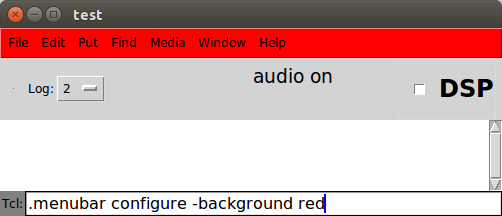
\includegraphics[scale=\Mysize]{tcl_prompt}
	\caption{Prompt tcl como \external}
\end{figure}

\begin{figure}[ht!]
	\centering
	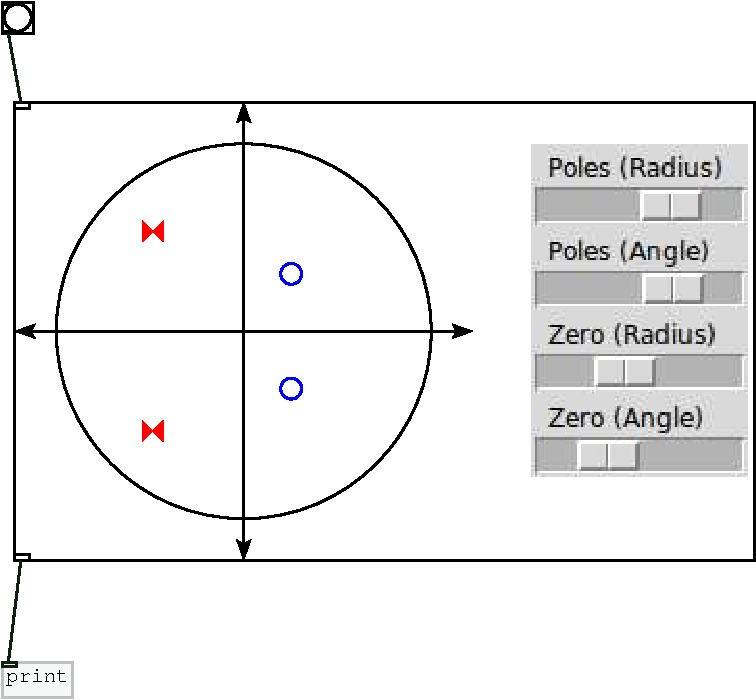
\includegraphics[scale=\Mysize]{filter_circle}
	\caption{Exemplo de \external com GUI TCL}
\end{figure}




% -----+-----+-----+-----+-----+-----+-----+-----+-----+-----+-----+-----+-----+
%      |     |     |     |     |     |     |     |     |     |     |     |     |
% -----+-----+-----+-----+-----+-----+-----+-----+-----+-----+-----+-----+-----+
\chapter{Plugins TCL}
Exemplos de plugins TCL: \url{http://puredata.info/docs/guiplugins/SimpleExamples/}

Every file that uses the xyz-plugin.tcl naming scheme and resides in the object search path of Pd is executed upon startup. More exactly, it is the pdtk\_pd\_startup function in pd-gui.tcl that calls the execution of startup plugins, in the following order:


\begin{lstlisting}
# META NAME My nifty plugin
# META DESCRIPTION Does all kinds of magic that may not be necessary for everyone
# META AUTHOR <John the Developer> johndev@mail.com

package require Tcl 8.5         # The minimum version of TCL that allows the plugin to run
package require Ttk             # If Tk or Ttk is needed
package require pdwindow 0.1    # Any elements of the Pd GUI that are required
                                # + require everything and all your script needs.
                                #   If a requirement is missing,
                                #   Pd will load, but the script will not.
\end{lstlisting}
\footnote{\url{http://puredata.info/docs/guiplugins/GUIPlugins/}}


Passando parâmentros

\begin{lstlisting}
    bind all <$::modifier-Key-a>      {menu_send %W selectall}
\end{lstlisting}

\section{Eventos do Pd}

http://puredata.info/docs/guiplugins/GuiPluginsAPI/

% -----+-----+-----+-----+-----+-----+-----+-----+-----+-----+-----+-----+-----+
%      |     |     |     |     |     |     |     |     |     |     |     |     |
% -----+-----+-----+-----+-----+-----+-----+-----+-----+-----+-----+-----+-----+
\section{Trocando dados entre C e TCL}

\begin{lstlisting}
   sys_gui(" if { [catch {pd}] } {proc pd {args} {pdsend [join $args " "]}}\n");
\end{lstlisting}

\todo{Mostrar problemas de um procedimento e 2 objetos}

\todo{Falar do expr?}




\part{\Externals em C}
% ----------------------------------------------------------------------------
% Introdução
% ----------------------------------------------------------------------------
 
\chapter{Introdução}

\example{
\begin{itemize}
\item \texttt{Makefile}
\end{itemize}
}


% -----+-----+-----+-----+-----+-----+-----+-----+-----+-----+-----+-----+-----+
%      |     |     |     |     |     |     |     |     |     |     |     |     |
% -----+-----+-----+-----+-----+-----+-----+-----+-----+-----+-----+-----+-----+
\section{Escrevendo \externals em C}

O código fonte do Pure Data é organizado de acordo com convenções de
programação orientada a objetos.
Para o desenvolvimento de \externals, é necessário seguir estas convenções e
fornecer ao ambiente uma nova classe com alguns métodos específicos, como
veremos mais adiante.
Para desenvolver para o Pure Data, é necessário importar o arquivo de cabeçalho
\texttt{m\_pd.h}\footnote{\url{http://pure-data.git.sourceforge.net/git/gitweb.cgi?p=pure-data/pure-data;a=blob\_plain;f=src/m\_pd.h;hb=HEAD}},
que contém definições de constantes, tipos e funções.

Uma boa fonte de informação é o tutorial de
\externals\footnote{\url{http://iem.at/pd/externals-HOWTO/pd-externals-HOWTO.pdf}}
escrito pelo IOHannes\footnote{\url{http://puredata.info/author/zmoelnig}}, um dos
programadores do Pure Data.
Apesar de ter utilizado este documento como ponto de partida, boa parte do que
está incluso no presente tutorial foi aprendido a partir da leitura do
código-fonte de \externals contidos no repositório oficial do Pure
Data\footnote{\url{http://pure-data.svn.sourceforge.net/viewvc/pure-data/trunk/externals/}}.

Navegando pelos códigos-fonte deste repositório você poderá notar que os programadores
que escreveram os externals que hoje estão disponível para o Pd seguiram estas convenções
e por isto a leitura destes códigos-fonte pode ser didática e simples.

Por esta razão, o primeiro conselho que damos para quem irá escrever \externals é seguir
estas convenções, mesmo que as mesmas não sejam a maneira como você está acostumado a 
programar deste jeito pois assim seu código também será didático e simples de entender.

Este tutorial não pretende cobrir os algoritmos de processamento de sinais mas explicar
como implementar estes algoritmos como objetos do Pd. Para processamento de sinais há
uma vasta bibliografia disponível que possui os algoritmos e o ferramental matemático
necessário para sua implementação.

% -----+-----+-----+-----+-----+-----+-----+-----+-----+-----+-----+-----+-----+
%      |     |     |     |     |     |     |     |     |     |     |     |     |
% -----+-----+-----+-----+-----+-----+-----+-----+-----+-----+-----+-----+-----+
\section{Organização do código-fonte e do objeto compilado}
\label{sec:organizacao}

Um novo \external corresponde a uma nova classe na arquitetura orientada a
objetos do Pure Data. Para que o carregamento da biblioteca dinâmica
em tempo de execução funcione corretamente, é necessário que o
arquivo binário produzido possua o mesmo nome que a classe correspondente ao
\external.

Para criar, por exemplo, um \external chamado ``passa-baixas'', podemos
escrever seu código-fonte em um arquivo chamado \texttt{passa-baixas.c}, e em
seguida compilar um objeto de biblioteca compartilhada chamado
\texttt{passa-baixas.pd\_linux}, no caso do sistema GNU/Linux.
Outras arquiteturas de sistema utilizam outras extensões para o nome do objeto com a
biblioteca compartilhada do \external, como por exemplo \texttt{.dll} (M\$
Windows), \texttt{.pd\_irix5} (SGI Irix) ou \texttt{.pd\_darwin} (Mac OS X).

\textbf{Importante:} O nome do arquivo com o código-fonte não possui formato
obrigatório, mas o nome do objeto compilado com a biblioteca dinâmica deve
sempre corresponder ao nome da classe, assim como sua extensão deve sempre
corresponder à arquitetura do sistema utilizado.

O mesmo cuidado é recomendado para os métodos que serão definidos internamente
no objeto. Os nomes de métodos que serão apresentados neste material seguem o padrão
encontrado no repositório do Pd.
É fortemente recomendado que o mesmo padrão seja utilizado em seu texto.

Para gerar a estrutura básica de um \external sugerimos utilizar o gerador de
\external disponível em \url{http://www.ime.usp.br/~fls/PDExternal-generator/PDExternal_generator.html}.

% -----+-----+-----+-----+-----+-----+-----+-----+-----+-----+-----+-----+-----+
%      |     |     |     |     |     |     |     |     |     |     |     |     |
% -----+-----+-----+-----+-----+-----+-----+-----+-----+-----+-----+-----+-----+
\section{Compilação}
\label{sec:compiling}

Para criar um objeto binário que pode ser carregado no Pure Data em tempo de
execução, primeiro compilamos o código fonte, criando assim um ou mais objetos
intermediários, e em seguida utilizamos um ligador (\emph{linker}) para criar
um objeto de biblioteca compartilhada.

No GNU/Linux, uma forma de realizar o processo
\texttt{example01.c} $\rightarrow$ \texttt{example01.o} $\rightarrow$
\texttt{example01.pd\_linux} é a seguinte:

\vspace{1em}
\begin{lstlisting}[caption=Compilação de um objeto]
EXTNAME=example01
cc -DPD -fPIC -Wall -o ${EXTNAME}.o -c ${EXTNAME}.c
ld -shared -lc -lm -o ${EXTNAME}.pd_linux ${EXTNAME}.o
rm ${EXTNAME}.o
\end{lstlisting}

A opção de compilação \texttt{-fPIC} resulta na criação de código binário que
roda independente de sua posição na memória, adequado para geração de
bibliotecas compartilhadas. A opção \texttt{-shared} passada para o ligador
determina a criação de uma biblioteca compartilhada.

Para facilitar a compilação, é interessante utilizar um \texttt{makefile}.
Os exemplos deste tutorial estão acompanhadas de um \texttt{makefile} encontrado
na seção de desenvolvedores do Pure
Data~\footnote{\url{http://puredata.info/docs/developer/MakefileTemplate}}.

Para compilar \externals no MacOS é necessário instalar o XCode.
Tem uma dezena de jeito de compilar pro Windows, usando o Mingw ou o C++ Builder.
Aqui\footnote{\url{http://puredata.hurleur.com/sujet-1029-problem-compiling-external-windows}}
temos exemplos e muitas discussões de como compilar externals no Windows.

\todo{Não testamos. Faltou coragem. Será que compensa testarmos isto tudo?}

\subsection{Debugando códigos}

Para verificar um erro, inicie o PD com seu patch de teste pelo terminal dentro do 
ambiente gdb com o comando

\begin{lstlisting}
gdb --args pd -path caminho-do-external

run
\end{lstlisting}
Caso o PD tenha algum problema em sua execução o GDB pode te ajudar a encontrá-lo.

Outros comandos básicos do gdb são \textbf{where} (que apresenta o arquivo e a linha onde
o erro ocorreu) e \textbf{list} (que mostra o código deste trecho).
Para navegar entre os arquivos, utilize \textbf{up} e \textbf{down}.
Para maiores informações, procure um tutorial sobre o gdb.

Além de debugar, pode ser útil verificar se o objeto está compilado corretamente.
Uma maneira de verificar isto é utilizar a ferramenta \texttt{nm} que lista os
símbolos de um objeto compilado.

\begin{lstlisting}
nm -D <external>.pd_linux
\end{lstlisting}

\subsection{Misturando código C e C++}

Existem algumas diferenças entre compiladores C e C++ que tornam a sintaxe das
linguagens incompatíveis, gerando resultados diferentes para um mesmo trecho
de código. Um exemplo disso que influencia o funcionamento de \externals no
Pure Data é a geração da tabela de símbolos dos objetos binários.

Compiladores C++ realizam um processo chamado \emph{name mangling} (ou
``dilaceramento de nomes''), que consiste em alterar o nome de funções,
estruturas, classes, etc, incluindo informações sobre o espaço de nomes do
objeto em questão. Isto resulta em nome diferentes gravados nas tabelas de
símbolos dos objetos binários, o que pode confundir o Pure Data no momento do
carregamento de um \external.

Para garantir que um compilador C++ gere nomes compatíveis com objetos
binários C, utilize a expressão \texttt{extern "C"} na frente dos nomes das
funções que serão chamadas pelo Pure Data:

\begin{lstlisting}[caption=Externalização de código C++]
extern "C" example01_setup(void);
extern "C" example01_new(void);
\end{lstlisting}




% ----------------------------------------------------------------------------
% O básico de um \external
% ----------------------------------------------------------------------------

\chapter{O básico de um \external}
\label{sec:basico}

\example{
\begin{itemize}
\item \texttt{helloworld.c}
\item \texttt{cowsay.c}
\item \texttt{example01.c}
\item \texttt{example03.c}
\item \texttt{example16.c}
\item \texttt{counter.c}
\end{itemize}
}

Escrever um \external significa seguir as recomendações da API. Peço ao leitor
bastante paciência pois este tutorial pretende andar um pouco devagar para
mostrar os passos da escrita de um \external.


% -----+-----+-----+-----+-----+-----+-----+-----+-----+-----+-----+-----+-----+
%      |     |     |     |     |     |     |     |     |     |     |     |     |
% -----+-----+-----+-----+-----+-----+-----+-----+-----+-----+-----+-----+-----+
\section{Um \external Hello World}

Como dissemos anteriormente, a arquitetura do Pure Data é organizada de acordo
com o paradigma de orientação a objetos: cada objeto gráfico do Pure Data
corresponde a uma instância de uma classe. Neste sentido, um \external está
associado a um conjunto de estruturas de dados que representam classes em C.
Veja que o conceito de objeto aqui não remete ao conceito de objetos de
linguagens de programação como Java ou C++.
Para cada classe é necessário haver métodos de instanciação, destruição,
processamento de sinais, tratamento de mensagens, etc.

A infraestrutura mínima para o funcionamento de um \external (de nome, digamos,
\texttt{<external>}) consiste em uma estrutura de dados para a representação
de uma classe, que deve ter nome \texttt{t\_<external>}, e dois métodos
obrigatórios, chamados \texttt{<external>\_setup()} e
\texttt{<external>\_new()}. Note que a convenção de nomes utilizada no Pure
Data é de que toda função deve ser nomeada da forma
\texttt{<contexto>\_<funcao>()}.

A estutura de dados que representa uma classe do Pure Data deve
obrigatoriamente possuir o primeiro atributo do tipo \texttt{t\_object}, no
qual é armazenado o objeto criado no momento da instanciação.
Outros atributos podem ser adicionados a esta estrutura de maneira que cada
instância da mesma classe possua os atributos necessários para seu
funcionamento.
Uma classe que acessa um arquivo, por exemplo, pode possuir como atributos uma
string para guardar o caminho e um inteiro para guardar o descritor do
arquivo.

Um exemplo de estrutura de dados para representação de uma classe chamada
\texttt{helloworld} consiste no seguinte:

\vspace{1em}
\begin{lstlisting}[caption=Estruturas de dados de um \external]
// ---------------------------------------------------
// Class definition
// ---------------------------------------------------
static t_class *helloworld_class;

// ---------------------------------------------------
// Data structure definition
// ---------------------------------------------------
typedef struct _helloworld {
   t_object x_obj;
} t_helloworld;
\end{lstlisting}

Tal objeto é passado para as funções que tratam mensagens e por isto tudo o que
for necessário para o funcionamento de seu external deve estar contido neste
objeto.
Aproveitamos para recomendar que isto inclua toda alocação e liberação de
memória que possa ser necessária.

Sempre que um \external é carregado pelo Pure Data, o método de nome
\texttt{<external>\_setup()} é executado. No exemplo dado acima, o Pure
Data irá procurar, no arquivo binário \texttt{example1.pd\_linux} que contém
a biblioteca compartilhada, o método de nome \texttt{example1\_setup(void)}.
Este método é utilizado para realizar a inicialização da classe, informando ao
Pure Data da existência de uma nova classe no sistema e associando a ela os
métodos de instanciação e destruição, além de outras informações:

\vspace{1em}
\begin{lstlisting}[caption=Método setup]
void helloworld_setup(void) {
   helloworld_class = class_new(
      gensym("helloworld"),          // Nome simbolico
      (t_newmethod) helloworld_new,  // Construtor
      (t_method) helloworld_destroy, // Destrutor
      sizeof (t_helloworld),         // Tamanho do objeto
      CLASS_NOINLET,                 // Flags com o tipo da classe
      0);                            // Argumentos do construtor
}
\end{lstlisting}

Dentro do método \texttt{<external>\_setup()} não há limite para o número de
classes a definir, de forma que é possível definir apenas uma classe (como no
exemplo helloworld.c) ou uma biblioteca inteira com várias classes (como no exemplo 3).
A introdução de uma nova classe no sistema é realizada pela função
\texttt{class\_new()}.
São parâmetros da função \texttt{class\_new()}:

\begin{itemize}
\item Nome simbólico da classe.
\item Método construtor de um objeto.
\item Método destrutor de um objeto.
\item Tamanho do espaço de dados dos atributos de um objeto.
\item Flags que definem a representação gráfica do objeto.
\item Tipos dos parâmetros a serem passados para o construtor quando da
      instanciação de um objeto (veja o próximo capítulo).
\end{itemize}

Os tipos de Flags aceitas para representar um objeto são:
\begin{itemize}
   \item CLASS\_DEFAULT - Para objetos padrões do PD com 1 inlet
   \item CLASS\_NOINLET - Objetos sem inlet ``Mágico''
   \item CLASS\_PD - Para objetos sem representação gráfica, como inlets
   \item CLASS\_GOBJ - Para objetos gráficos como arrays e graphs
   \item CLASS\_PATCHABLE - Para objetos internos do PD como ``message'' ou ``text''
\end{itemize}

É necessário terminar a lista de tipos de parâmetros com um número inteiro 0,
para indicar ao Pure Data que a lista de tipos terminou.
Consulte a documentação da função \texttt{class\_new()} para mais
detalhes\footnote{\url{http://pdstatic.iem.at/externals-HOWTO/node9.html\#SECTION00092100000000000000}}.

O método \texttt{<external>\_new()}, que foi associado como método de
instanciação de objetos na chamada de \texttt{class\_new()}, realiza a
instanciação de objetos propriamente dita.
Neste método, além da instanciação de um novo objeto através da função
\texttt{pd\_new()}, é possível definir os
valores dos atributos da estrutura de dados da classe e também inicializar
quaisquer outros contextos que sejam necessários, como por exemplo abrir
arquivos, preencher vetores, alocar memória, etc.

\vspace{1em}
\begin{lstlisting}[caption=Construtor de uma classe]
// ---------------------------------------------------
// Construtor da classe
// ---------------------------------------------------
void * helloworld_new(void){
   t_helloworld *x = (t_helloworld *) pd_new(helloworld_class);
   // Something else?
   return (void *) x;
}
\end{lstlisting}

Após a criação da estrutura de dados dos métodos da forma mencionada acima, a
compilação realizada da forma descrita na seção \ref{sec:compiling}, e a
criação do objeto no Pure Data como descrito na seção \ref{sec:using}, o
resultado pode ser visto na figura \ref{fig:example1}.

\grafico{example1}{Nosso primeiro \external do PD. Ainda inútil. :-$\left.\right)$}

% -----+-----+-----+-----+-----+-----+-----+-----+-----+-----+-----+-----+-----+
%      |     |     |     |     |     |     |     |     |     |     |     |     |
% -----+-----+-----+-----+-----+-----+-----+-----+-----+-----+-----+-----+-----+
\section{Uma biblioteca simples}

Um mesmo método \texttt{<external>\_setup()} pode definir várias classes
diferentes. A isto damos o nome de biblioteca. Neste cenário, o método
\texttt{<external>\_setup()} possui o mesmo nome do arquivo com a biblioteca,
mas cada classe podem ter um nome diferente (veja o exemplo 3).

\vspace{1em}
\begin{lstlisting}[caption=Exemplo de arquivo com duas classes]
void example3_setup(void) {
  post("Initializing my library");

  myobj1_class = class_new(
    gensym("myobj1"),
    (t_newmethod) myobj1_new, // Constructor
    0,
    sizeof (t_myobj1),
    CLASS_NOINLET,
    0);
  class_sethelpsymbol(myobj1_class, gensym("myobj1-help"));

  myobj2_class = class_new(
    gensym("myobj2"),
    (t_newmethod) myobj2_new, // Constructor
    0,
    sizeof (t_myobj2),
    CLASS_NOINLET,
    0);
  class_sethelpsymbol(myobj2_class, gensym("myobj2-help"));
}
\end{lstlisting}

Se o arquivo foi preenchido corretamente, compilado corretamente e adicionado
ao caminho do PureData, teremos o resultado visto na figura \ref{fig:exemplo3}.

\grafico{example3}{Nosso segundo \external do PD. Ainda inútil. :-$\left.\right)$}

Caso seu objeto não tenha funcionado, verifique se vc utilizou o parâmetro 
\texttt{-lib example03} para executá-lo.


Apesar de este tipo de biblioteca ser bastante utilizado no código-fonte do PD,
é recomendado separar os \external em arquivos individuais para simplificar
a leitura e manutenção do código-fonte.
Sendo assim, é recomendado que o \external ``myobj1'' esteja em um arquivo
chamado ``myobj1.c'' e que o mesmo seja feito com o \external ``myobj2''.

% -----+-----+-----+-----+-----+-----+-----+-----+-----+-----+-----+-----+-----+
%      |     |     |     |     |     |     |     |     |     |     |     |     |
% -----+-----+-----+-----+-----+-----+-----+-----+-----+-----+-----+-----+-----+
\section{Outras informações de um \external}

Dentro do Pure Data, um clique com o botão direito em um objeto abre um menu
no qual uma das opções é \texttt{Ajuda}. Quando esta opção é selecionada, o
Pure Data abre um patch associado ao objeto, que deve conter instruções e
exemplos de uso. Por padrão, o Pure Data procura um arquivo com o mesmo nome
que o external (acrescido da extensão \texttt{-help.pd}) no diretório padrão de
documentação (\texttt{doc/5.reference}). Para associar um arquivo diferente do
padrão, basta utilizar a função \texttt{class\_sethelpsymbol}:

\vspace{1em}
\begin{lstlisting}[caption=Definição de arquivo de help]
class_sethelpsymbol(myclass_class, gensym("my_class-help"));
\end{lstlisting}

Um objeto pode ainda ter outros nomes (\emph{aliases}). Para definir isto
podemos utilizar a função \texttt{class\_addcreator()}. Veja o exemplo:

\vspace{1em}
\begin{lstlisting}[caption=Definição de alias para um objeto]
class_addcreator((t_newmethod)medusa_new, gensym("med"), 0);
\end{lstlisting}

Exemplos comuns de aliases são os objetos [send], [receive] e [trigger], que
podem ser instanciados pelos aliases [s], [r] e [t] respectivamente.

% -----+-----+-----+-----+-----+-----+-----+-----+-----+-----+-----+-----+-----+
%      |     |     |     |     |     |     |     |     |     |     |     |     |
% -----+-----+-----+-----+-----+-----+-----+-----+-----+-----+-----+-----+-----+
\section{Variáveis globais}

É possível utilizar variáveis globais para armazenar dados de um \external.
Estas variáveis são visíveis para todas as intâncias de objetos do \external e
todas podem alterar seus valores.
Isto pode ser útil ou um desastre (veja o exemplo16).
Por exemplo, cada instância do \external \texttt{example16}
definido a partir do código a seguir incrementa em uma unidade o valor do
contador, como pode ser visto na figura \ref{fig:example16}:

\vspace{1em}
\begin{lstlisting}[caption=Exemplo de uma variável global]
int count = 0;

void * example16_new(void) {
    t_example16 *x = (t_example16 *) pd_new(example16_class);
    post("Counter value: %d",count);
    count++;
    return (void *) x;
}
\end{lstlisting}

\grafico{example16}{Repare na saída da janela principal.}

Caso isto não seja desejável, o ideal é incluir as variáveis dentro da
estrutura do objeto.
Assim, neste exemplo cada instância terá seu próprio contador:

\vspace{1em}
\nopagebreak{
\begin{lstlisting}[caption=Objeto contador]
static t_class *counter_class;

typedef struct _counter {
   t_object x_obj;
   t_float counter;
   t_outlet * x_outlet_output_float;
} t_counter;

void * counter_new(void){
   t_counter *x = (t_counter *) pd_new(counter_class);
   x->counter = 0;
   x->x_outlet_output_float = outlet_new(&x->x_obj, gensym("float"));
   return (void *) x;
}
\end{lstlisting}

Vale notar que adicionar a estrutura de dados do \external os atributos
necessários para seu funcionamento é a abordagem padrão para o desenvolvimento.
É recomendado que o compartilhamento de dados entre dois objetos ocorra pela
troca de mensagem e não por variáveis globais.



% ----------------------------------------------------------------------------
% OS TIPOS DE DADOS DO PD
% ----------------------------------------------------------------------------
\chapter{Os tipos de dados do PD}

Uma vez que o Pure Data é utilizado em diversas plataformas, muitos tipos
comuns de variáveis, como \texttt{int}, são redefinidos. Para escrever um
\external que seja portável para qualquer plataforma, é razoável que você
utilize os tipos providos pelo Pure Data. Como dissemos na seção
\ref{sec:organizacao}, para escrever um \external, é necessário incluir o
arquivo \texttt{m\_pd.h} que possui definições de constantes (versão do Pure
Data, sistema operacional, compilador, etc), estruturas, assinaturas de
funções e tipos de dados.

Existem muitos tipos predefinidos que devem fazer a vida do programador mais
simples. Em geral, os tipos do pd têm nome iniciado por \texttt{t\_}.

\begin{center}
\begin{tabular}{|l|l|}
\hline
tipo do pd & descrição \\
\hline
\texttt{t\_atom}      & átomo \\
\texttt{t\_float}     & valor de ponto flutuante \\
\texttt{t\_symbol}    & símbolo \\
\texttt{t\_gpointer}  & ponteiro (para objetos gráficos) \\
\texttt{t\_int}       & valor inteiro \\
\texttt{t\_signal}    & estrutura de um sinal \\
\texttt{t\_sample}    & valor de um sinal de áudio (ponto flutuante) \\
\texttt{t\_outlet}    & \emph{outlet} de um objeto \\
\texttt{t\_inlet}     & \emph{inlet} de um objeto \\
\texttt{t\_object}    & objeto gráfico \\
\texttt{t\_class}     & uma classe do pd \\
\texttt{t\_method}    & um método de uma classe \\
\texttt{t\_newmethod} & ponteiro para um construtor (uma função \texttt{\_new}) \\
\hline
\end{tabular}
\end{center}

% -----+-----+-----+-----+-----+-----+-----+-----+-----+-----+-----+-----+-----+
%      |     |     |     |     |     |     |     |     |     |     |     |     |
% -----+-----+-----+-----+-----+-----+-----+-----+-----+-----+-----+-----+-----+
\section{Símbolos}

Um símbolo corresponde a um valor constante de uma \emph{string}, ou seja,
uma sequência de letras que formam uma palavra única.

Cada símbolo é armazenado em uma tabela de busca por razões de performance. A
função \texttt{gensym(char *)} procura por uma string em uma tabela de busca e
retorna o endereço daquele símbolo. Se a string não foi encontrada na tabela,
um novo símbolo é adicionado.

Estes símbolos serão usados para várias coisas como para criar e associar mensagens 
entre objetos, definir ações esperadas para mensagens recebidas por inlets, criar 
comunicação entre a GUI e o Pd, entre outras.

Para imprimir, por exemplo, o valor de uma String contida em um \texttt{t\_symbol} é
necessário acessar sua propriedade \texttt{s\_name}.

Exemplo:

\begin{lstlisting}[caption=Imprimindo o texto de um símbolo]
   printf("%s\n", my_symbol->s_name);
\end{lstlisting}

% -----+-----+-----+-----+-----+-----+-----+-----+-----+-----+-----+-----+-----+
%      |     |     |     |     |     |     |     |     |     |     |     |     |
% -----+-----+-----+-----+-----+-----+-----+-----+-----+-----+-----+-----+-----+
\section{Mensagens}
\label{sec:mensagens}

Dados que não correspondem a áudio são distribuídos via um sistema de
mensagens.
Cada mensagem é composta de um ``seletor" e uma lista de átomos.

\subsection{Átomos}
\label{sec:atomos}

Um átomo é um tipo de dado do PD que possui um valor e uma identificação.
Os tipos de átomo mais utilizados são:

\begin{itemize}
\item \texttt{A\_FLOAT}: um valor numérico (de ponto flutuante).
\item \texttt{A\_SYMBOL}: um valor simbólico (string).
\item \texttt{A\_POINTER}: um ponteiro.
\end{itemize}


Valores numéricos são sempre considerados valores de ponto flutuante
(\texttt{t\_float}), mesmo que possam ser exibidos como valores inteiros.

Átomos do tipo \texttt{A\_POINTER} não são muito importantes (para \externals
simples).

O tipo de um átomo \texttt{a} é armazenado no elemento da estrutura
\texttt{a.a\_type}.

Outros tipos de átomo definidos no arquivo \texttt{m\_pd.h} são:

\begin{itemize}
\item \texttt{A\_NULL},
\item \texttt{A\_FLOAT},
\item \texttt{A\_SYMBOL},
\item \texttt{A\_POINTER},
\item \texttt{A\_SEMI},
\item \texttt{A\_COMMA},
\item \texttt{A\_DEFFLOAT},
\item \texttt{A\_DEFSYM},
\item \texttt{A\_DOLLAR},
\item \texttt{A\_DOLLSYM},
\item \texttt{A\_GIMME},
\item \texttt{A\_CANT}
\end{itemize}

Nem todos estes átomos são utilizados no desenvolvimento de \externals e alguns
são representações internas do PD para símbolos reservados como vírgula, cifrão
ou nulo.
Assim, se um objeto precisa passar para outro objeto um valor nulo, um cifrão ou
vírgula, estes tipos devem ser utilizado.

A manipulação de átomos pode ser feita pelas seguintes funções:

\subsubsection{\texttt{SETFLOAT}}
\texttt{SETFLOAT(atom, f)}

Esta macro define o tipo do átomo como \texttt{A\_FLOAT} e armazena no mesmo o valor de f.
É necessário passar um ponteiro para o átomo.

\subsubsection{\texttt{SETSYMBOL}}
\texttt{SETSYMBOL(atom, s)}

Esta macro define o tipo do átomo como \texttt{A\_SYMBOL} e armazena no mesmo um ponteiro
para o símbolo s.
É necessário passar um ponteiro para o átomo.

\subsubsection{\texttt{SETPOINTER}}
\texttt{SETPOINTER(atom, pt)}

Esta macro define o tipo do átomo como \texttt{A\_POINTER} e armazena no mesmo o ponteiro
pt.
É necessário passar um ponteiro para o átomo.

\subsubsection{\texttt{atom\_getfloat}}
\texttt{t\_float atom\_getfloat(t\_atom *a)}

Se o átomo for do tipo \texttt{A\_FLOAT}, retorna o valor do float, caso contrário,
retorna 0.0.

\subsubsection{\texttt{atom\_getfloatarg}}
\texttt{t\_float atom\_getfloatarg(int which, int argc, t\_atom *argv)}

Se o tipo do átomo encontrado na lista de átomos argv, de tamanho argc e na
posição which for \texttt{A\_FLOAT}, retorna o valor deste átomo.
Caso contrário, retorna 0.0.

\subsubsection{\texttt{atom\_getint}}
\texttt{t\_int atom\_getint(t\_atom *a)}

Se o átomo for do tipo \texttt{A\_INT}, retorna o valor inteiro, caso contrário,
retorna 0.

\subsubsection{\texttt{atom\_getintarg}}
\texttt{t\_int atom\_getintarg(int which, int argc, t\_atom *argv)}

Se o tipo do átomo encontrado na lista de átomos argv, de tamanho argc e na
posição which for \texttt{A\_INT}, retorna o valor deste átomo.
Caso contrário, retorna 0.

\subsubsection{\texttt{atom\_getsymbol}}
\texttt{t\_symbol atom\_getsymbol(t\_atom *a)}

Se o átomo for do tipo \texttt{A\_SYMBOL}, retorna um ponteiro para este símbolo, caso
contrário, retorna ``0''.

\subsubsection{\texttt{atom\_getsymbolarg}}
\texttt{t\_symbol atom\_getsymbolarg(int which, int argc, t\_atom *argv)}

Se o tipo do átomo encontrado na lista de átomos argv, de tamanho argc e na
posição which for \texttt{A\_SYMBOL}, retorna um ponteiro para este símbolo.
Caso contrário, retorna ``0''.

\subsubsection{\texttt{atom\_gensym}}
\texttt{t\_symbol *atom\_gensym(t\_atom *a)}

Se o átomo for do tipo \texttt{A\_SYMBOL}, retorna um ponteiro para este símbolo.
Átomos de outros tipos são convertidos de maneira ``razoável'' em string,
adicionados na tabela de símbolos, e um ponteiro para este símbolo é retornado.

\subsubsection{\texttt{atom\_string}}
\texttt{void atom\_string(t\_atom *a, char *buf, unsigned int bufsize)}

Converte um átomo em uma string (char *) previamente alocada e de tamanho bufsize.

\subsection{Seletores}

Um seletor é um símbolo que define o tipo de uma mensagem. Existe cinco
seletores pré-definidos:

\begin{itemize}
  \item \texttt{bang}: rotula um gatilho de evento. Uma mensagem de
    \texttt{bang} consiste somente do seletor e não contém uma lista de átomos.
  \item \texttt{float} rotula um valor numérico. A lista de uma mensagem
    \texttt{float} contém um único átomo de tipo \texttt{A\_FLOAT}.
  \item \texttt{symbol} rotula um valor simbólico. A lista de uma mensagem
    \texttt{symbol} consiste em um único átimo do tipo \texttt{A\_SYMBOL}.
  \item \texttt{pointer} rotula um valor de ponteiro. A lista de uma mensagem do
    tipo \texttt{pointer} contém um único átimo do tipo \texttt{A\_POINTER}.
  \item \texttt{list} rotula uma lista de um ou mais átomos de tipos arbitrários.
\end{itemize}

Uma vez que os símbolos para estes seletores são utilizados com frequência,
seu endereço na tabela de símbolos pode ser utilizado diretamente, sem a
necessidade da utilização de \texttt{gensym}:

\begin{center}
\begin{tabular}{|l|l|l|}
\hline
  seletor & rotina de busca & endereço de busca \\
\hline
  \texttt{bang} & \texttt{gensym("bang")} & \texttt{\&s\_bang} \\
  \texttt{float} & \texttt{gensym("float")} & \texttt{\&s\_float} \\
  \texttt{symbol} & \texttt{gensym("symbol")} & \texttt{\&s\_symbol} \\
  \texttt{pointer} & \texttt{gensym("pointer")} & \texttt{\&s\_pointer} \\
  \texttt{list} & \texttt{gensym("list")} & \texttt{\&s\_list} \\
  \texttt{--}  (signal) & \texttt{gensym("signal")} & \texttt{\&s\_signal} \\
\hline
\end{tabular}
\end{center}

Outros seletores também podem ser utilizados. A classe receptora tem que
prover um médodo para um seletor específico ou para \texttt{anything}, que
corresponde a qualquer seletor arbitrário.

Mensagens que não possuem seletor explícito e começam com um valor numérico
são reconhecidas automaticamente como mensagens \texttt{float} (se consistirem
de apenas um átomo) ou como mensagens \texttt{list} (se forem compostas de
diversos átomos).

Por exemplo, as mensagens \texttt{12.429} e \texttt{float 12.429} são
idênticas. Da mesma forma, as mensagens \texttt{list 1 para voce} é idêntica a
\texttt{1 para voce}.

\todo{Cabe escrever sobre binbuf?}

% ----------------------------------------------------------------------------
% CONSTRUTOR E DESTRUTOR
% ----------------------------------------------------------------------------
\chapter{Construtor e destrutor}

\example{
\begin{itemize}
\item \texttt{example02.c}
\item \texttt{example09.c}
\end{itemize}
}

Um objeto em PD pode precisar de determinados parâmetros para ser iniciado.
Por exemplo, para criar um oscilador é necessário passar para este objeto a
frequência que o mesmo irá funcionar.
Assim, o objeto recebe um parâmetro como, por exemplo, [osc~ 440].
Para receber parâmetros na criação de um objeto é necessário informar o PD do mesmo.
Para isto, é necessário tanto informar os parâmetros na definição da classe quanto
definir corretamente a assinatura da função do construtor.
Estes parâmetros são ilustrados abaixo.

\grafico{example2}{\external recebendo parâmetros. Note a tela de saída no fundo da imagem.}


% -----+-----+-----+-----+-----+-----+-----+-----+-----+-----+-----+-----+-----+
%      |     |     |     |     |     |     |     |     |     |     |     |     |
% -----+-----+-----+-----+-----+-----+-----+-----+-----+-----+-----+-----+-----+
\section{Tipos de parâmetros}

Os tipos de parâmetros aceitos para o construtor com checagem de tipo são:
\begin{itemize}
   \item \texttt{A\_DEFSYMBOL} para Strings
   \item \texttt{A\_DEFFLOAT} para números
\end{itemize}

Por questões de implementação, o PD pode verificar apenas 5 parâmetros com tipo.
Para passar mais parâmetros ao construtor é necessário utilizar um outro tipo
de parâmetro:

\begin{itemize}
   \item \texttt{A\_GIMME} para qualquer tipo de parâmetro
\end{itemize}

Caso este tipo seja utilizado, o construtor deverá receber uma lista de átomos
de tamanhos e tipos arbitrários e não faz a verificação de tipos.

A assinatura do construtor para receber ester parâmetros são:

\begin{lstlisting}[caption=Assinatura do construtor]
void *myclassnew(void) // Construtor sem parametros
void *myclassnew(t_symbol *arg)  // Para parametro tipo A_DEFSYMBOL
void *myclassnew(tfloatarg arg) // Para parametro tipo A_DEFFLOAT
void *myclass_new(t_symbol *s , int argc , t_atom * argv) // Para A_GIMME
\end{lstlisting}

% -----+-----+-----+-----+-----+-----+-----+-----+-----+-----+-----+-----+-----+
%      |     |     |     |     |     |     |     |     |     |     |     |     |
% -----+-----+-----+-----+-----+-----+-----+-----+-----+-----+-----+-----+-----+
\section{Construtor}

Parâmetros de inicialização no construtor podem permitir que inicializemos o
external com determinados valores. Isto é feito definindo os parâmetros no
métodos \texttt{class\_new()} quanto na definição da função construtora. (Veja o
exemplo02).

\begin{lstlisting}[caption=Passagem de parâmetro para o construtor]
// Constructos of the class
void * example02_new(t_floatarg arg1, t_symbol * arg2) {
    t_example02 *x = (t_example02 *) pd_new(example02_class);
    post("First arg: %f", arg1);
    post("Second arg: %s", arg2->s_name);
    return (void *) x;
}

void example02_setup(void) {
    example02_class = class_new(gensym("example02"),
            (t_newmethod) example02_new, // Constructor
            0,
            sizeof (t_example02),
            CLASS_NOINLET,
            A_DEFFLOAT, // First Constructor parameter
            A_DEFSYMBOL, // Second Constructor parameter
            0);
}
\end{lstlisting}

Notem que os parâmetros são definidos com um tipo e são recebidos com outro.
Como explicado na seção \ref{sec:mensagens}, todos os dados que não
correspondem a sinais de áudio são transmitidos como mensagens, compostas de
átomos.
Para ver os tipos de átomo que podem ser utilizados na passagem de parâmetros,
veja a seção \ref{sec:atomos}.

Para aceitar qualquer tipo de átomo na passagem de um parâmetro específico,
utilize o tipo de átomo \texttt{A\_GIMME} (veja o exemplo09).

\begin{lstlisting}[caption=Objeto que recebe qualquer tipo de parâmetro]
// Constructor of the class
void * example09_new(t_symbol *s, int argc, t_atom * argv) {
   t_example09 *x = (t_example09 *) pd_new(example09_class);
   post("%d parameters received",argc);
   return (void *) x;
}

void example09_setup(void) {
   example09_class = class_new(gensym("example09"),
     (t_newmethod) example09_new, // Constructor
     (t_method) example09_destroy, // Destructor
     sizeof (t_example09),
     CLASS_NOINLET,
     A_GIMME, // Allows various parameters
     0); // LAST argument is ALWAYS zero
}
\end{lstlisting}

Quando utilizamos o tipo de átomo \texttt{A\_GIMME} o método construtor
funciona como uma função \texttt{main()} em C: ela recebe os parâmetros
\texttt{argc}, que indica o número de átomos na lista, e \texttt{*argv}, que
aponta para a lista de átomos de fato. Veja o exemplo na figura
\ref{fig:example9}.

\grafico{example9}{Diferente da linguagem C, o primeiro parâmetro não é o nome do external.}

Neste caso, diferentemente da função main na linguagem C, o primeiro parâmetro
não é o nome do external.
O nome do external é o primeiro parâmetro recebido pela função, em nosso exemplo,
``t\_symbol *s''.

% -----+-----+-----+-----+-----+-----+-----+-----+-----+-----+-----+-----+-----+
%      |     |     |     |     |     |     |     |     |     |     |     |     |
% -----+-----+-----+-----+-----+-----+-----+-----+-----+-----+-----+-----+-----+
\section{Validando parâmetros no construtor}

Note que o Pure Data não obriga que o usuário passe parâmetros para o objeto.
Todo construtor, independentemente de como ele está definido, aceita
sua instanciação vazia.
Cabe ao programador verificar se os parâmetros recebidos são em quantidade,
tipo e valor esperado e, caso não seja, abortar a construção do objeto e não
retornar sua instância.

\begin{lstlisting}[caption=Validando parâmetros na construção de um objeto]
// Constructor of the class
void * example09_new(t_symbol *s, int argc, t_atom * argv) {
   t_example09 *x = (t_example09 *) pd_new(example09_class);
   post("External name: %s", s->s_name);
   post("%d parameters received",argc);
   if(argc < 1){
      post("Please, gimme some parameters!");
      return NULL;
   }
   if(argv[0]->a_type != A_FLOAT{
      post("Gimme a float!");
      return NULL;
   }
   return (void *) x;
}
\end{lstlisting}

Como podemos verificar no exemplo código acima, caso não seja passado um parâmetro
do tipo float para o example09 o mesmo não irá retornar uma instância do objeto
e apresentará a mensagem de que parâmetros devem ser passado ao objeto.

% -----+-----+-----+-----+-----+-----+-----+-----+-----+-----+-----+-----+-----+
%      |     |     |     |     |     |     |     |     |     |     |     |     |
% -----+-----+-----+-----+-----+-----+-----+-----+-----+-----+-----+-----+-----+
\section{Outras tarefas para o construtor}

Como deve-se saber, não é aconselhável alocar memória durante o bloco de
processamento de sinais quando trabalhamos com processamento em tempo real.
Por esta razão, é aconselhável alocar a memória de variáveis que iremos utilizar
em nosso \external no construtor.

Um exemplo de dados que deve ser alocado e instanciado no construtor seria uma
tabela seno para criar um oscilador por consulta a tabela.

\begin{lstlisting}[caption=Função para a alocação de memória]
void *getbytes(size_t nbytes);
\end{lstlisting}

A alocação de memória deve ser feita preferencialmente pela função \texttt{getbytes}.
Esta função utiliza internamente a função padrão \texttt{malloc} porém é portável
para os sistemas operacionais onde o PD funciona.

Outra tarefa que pode ser realizada pelo construtor é a criação de iolets
passivos.
Tal funcionalidade será coberta no próximo capítulo deste documento.

% -----+-----+-----+-----+-----+-----+-----+-----+-----+-----+-----+-----+-----+
%      |     |     |     |     |     |     |     |     |     |     |     |     |
% -----+-----+-----+-----+-----+-----+-----+-----+-----+-----+-----+-----+-----+
\section{Destrutor}

O destrutor de uma classe permite liberar alguma memória eventualmente alocada
pelo construtor ou por outras funções do \external (veja o exemplo 07).

\begin{lstlisting}[caption=Exemplo de destrutor]
// Destroy the object
void example09_destroy(t_example09 *x) {
  post("You say good bye and I say hello");
}

void example09_setup(void) {
   example09_class = class_new(gensym("example09"),
     (t_newmethod) example09_new, // Constructor
     (t_method) example09_destroy, // Destructor
     sizeof (t_example09),
     CLASS_NOINLET,
     A_GIMME, // Allows various parameters
     0); // LAST argument is ALWAYS zero
}
\end{lstlisting}

De maneira análoga a alocação de memória, o PD também disponibiliza uma função
portável para a liberação de memória.
A liberação da memória pode ser feita utilizando a função \texttt{freebytes()}
definida na API do Pure Data.
Tal função deve chamar internamente a função padrão \texttt{free} sendo, porém,
portável entre diferentes sistemas operacionais.

\begin{lstlisting}
void freebytes(void *x, size_t nbytes)
\end{lstlisting}

% ----------------------------------------------------------------------------
% INLETS E OUTLETS
% ----------------------------------------------------------------------------

\chapter{Inlets e outlets}

\example{
\begin{itemize}
\item \texttt{inverter.c}
\item \texttt{example04.c}
\item \texttt{evenodd.c}
\item \texttt{example05.c}
\item \texttt{example06.c}
\item \texttt{example08.c}
\item \texttt{yourclass.c}
\item \texttt{multiplus.c}
\item \texttt{outlet\_dinamico.c}
\end{itemize}
}

Os objetos que criamos até agora são inúteis.
Não servem para nada, pois não se comunicam com outros objetos nem modificam
sinais de áudio.
Para dar utilidade a um \external, é necessário que ele comunique com outros objetos
do Pure Data.
Isto é feito por meio de \emph{inlets} e \emph{outlets}, portas
de entrada e saída (respectivamente) de sinais de áudio e/ou mensagens.

Neste capítulo vamos tratar exclusivamente de inlets e outlets de mensagens.
Entre os inlets de mensagem há os tipos passivos e ativos, que os usuários
costumam chamar de inlets frios e quentes.
Inlets \textbf{passivos} são inlets cujo valor recebido é associada diretamente
a um atributo do objeto.
São chamados de passivos pois a alteração do seu valor não resulta na chamada
de um método e a atribuição do valor recebido ao atributo do objeto é feita
automaticamente.
Inlets \textbf{ativos}, por outro lado, são associados a
funções e permitem a execução de uma função arbitrária quando um valor é
recebido no inlet.

As mensagens passadas para o objeto em seus inlets ocorre por passagem de valor
para o caso de inteiros e por passagem de parâmetros para os demais tipos.
Por isto, é necessário cuidado ao manipular tais mensagens pois a alteração do
valor de um ponteiro implica na alteração do mesmo em todos os objetos que o
recebe.
Veja o exemplo \texttt{inverter.c}.
Neste exemplo o valor de um Symbol é alterado e resulta no mesmo invertido.
Caso você inverta este valor, salve o patch, feche-o e abra-o novamente, encontrará o
valor deste símbolo invertido, conforme apresentado nas Figuras \ref{fig:inverter} e
\ref{fig:inverter2}.

\grafico{inverter}{Alteração de uma mensagem recebida.}

\grafico{inverter2}{Alteração de uma mensagem recebida, ao reabrir.}


% -----+-----+-----+-----+-----+-----+-----+-----+-----+-----+-----+-----+-----+
%      |     |     |     |     |     |     |     |     |     |     |     |     |
% -----+-----+-----+-----+-----+-----+-----+-----+-----+-----+-----+-----+-----+
\section{Inlets ativos}

Um inlet ativo sempre recebe mensagens no primeiro inlet do objeto e por isto
o mesmo deve ser utilizado com a classe do tipo \texttt{CLASS\_DEFAULT}.
Estes inlets são sempre associados a uma função.
A criação de um inlet ativo define o tipo do átomo que o inlet receberá (veja o
exemplo 05 e o resultado na figura \ref{fig:inlet-ativo}).

\begin{lstlisting}[caption=Exemplo de objeto com inlet ativo]
// all inlet-methods receive the object as their first argument.
void example05_bang(t_example05 *x) { 
  post("BANGED!");
}

void example05_anything(t_example05 *x, t_symbol *s, int argc, t_atom *argv){
  post("ANYTHING!");
}

void example05_setup(void) {
  example05_class = class_new(gensym("example05"),
    (t_newmethod) example05_new, // Constructor
    0, 
    sizeof (t_example05),
    CLASS_DEFAULT,
    0); // LAST argument is ALWAYS zero
  class_addbang(example05_class, example05_bang);
  class_addanything(example05_class, example05_anything);
}
\end{lstlisting}

Neste exemplo, definimos duas funções associadas ao primeiro inlet, uma para
receber uma mensagem \texttt{bang} e outra para receber qualquer tipo de dado.
O resultado desta implementação pode ser vista na Figura \ref{fig:example5}.

\grafico{example5}{Inlets ativos.}

Abaixo, a tabela com os métodos que criam inlets ativos,
e assinaturas possíveis para funções associadas a cada tipo:

\begin{center}
\begin{tabular}{|l|l|}
\hline
método do pd para criar inlet ativo & assinatura para o método associado ao
inlet \\
\hline
\texttt{class\_addbang(t\_class *c, t\_method fn);}   & \texttt{my\_b(t\_myt *x);} \\
\texttt{class\_addfloat(t\_class *c, t\_method fn);}  & \texttt{my\_f(t\_myt *x, t\_floatarg f);} \\
\texttt{class\_addsymbol(t\_class *c, t\_method fn);} & \texttt{my\_s(t\_myt *x,t\_symbol *s);} \\
\texttt{class\_addpointer(t\_class *c, t\_method fn);}& \texttt{my\_p(t\_myt *x, t\_gpointer *pt);} \\
\texttt{class\_addlist(t\_class *c, t\_method fn);}   & \texttt{my\_l(t\_myt *x, t\_symbol *s, int argc, t\_atom *argv);} \\
\texttt{class\_addanything(t\_class *c, t\_method fn);}& \texttt{my\_a(t\_mydata *x, t\_symbol *s, int argc, t\_atom *argv);} \\
\hline
\end{tabular}
\end{center}

% -----+-----+-----+-----+-----+-----+-----+-----+-----+-----+-----+-----+-----+
%      |     |     |     |     |     |     |     |     |     |     |     |     |
% -----+-----+-----+-----+-----+-----+-----+-----+-----+-----+-----+-----+-----+
\section{Mensagens para o primeiro inlet}

Da mesma maneira que é possível mapear os tipos de dados recebidos no primeiro
inlet para funções, também é possível definir tipos de mensagens separadamente.
Isto é feito através da função \texttt{add\_method()} (veja o exemplo 08).
Esta função permite que a mensagem possua um identificador com seu tipo e outros
dados que acompanham esta mensagem.

\begin{lstlisting}[caption=Passagem de mensagens para o primeiro inlet]
// Constructor of the class
void * example08_new(void) {
  t_example08 *x = (t_example08 *) pd_new(example08_class);
  return (void *) x;
}

void example08_start(t_example08 *x){
  post("START / BANG");
}

void example08_open(t_example08 *x, t_symbol *s){
  post("open %s",s->s_name);
}


void example08_alfa(t_example08 *x, t_floatarg f){
  post("ALFA VALUE %f",f);
}

void example08_setup(void) {
  example08_class = class_new(gensym("example08"),
    (t_newmethod) example08_new, // Constructor
    (t_method) example08_destroy, // Destructor
    sizeof (t_example08),
    CLASS_DEFAULT,
    0); // LAST argument is ALWAYS zero
  // All these messages will be received by the first left inlet
  class_addmethod(example08_class, (t_method) example08_start, 
    gensym("start"), 0); // two messages, the same function
  class_addmethod(example08_class, (t_method) example08_start, 
    gensym("bang"),  0); // may be "start" or "bang" messages
  class_addmethod(example08_class, (t_method) example08_open,  
    gensym("open"),  A_DEFSYMBOL,0);
  class_addmethod(example08_class, (t_method) example08_alfa,  
    gensym("alfa"), A_DEFFLOAT,0); 
}
\end{lstlisting}

A listagem acima mostra que as mensagens \texttt{bang} e \texttt{start} são
associadas ao mesmo método.
Além disto, a mensagem \texttt{open} recebe um texto como parâmetro e a mensagem
\texttt{alfa} recebe um float como parâmetro.
Como no construtor, a função \texttt{class\_addmethod} pode receber uma lista de
e receber um valor zero como último argumento.

Desta forma não precisamos tratar a mensagem que o inlet recebe mas definí-las
de antemão e criar funções que mapeiem a mensagem recebida.
Veja a Figura \ref{fig:example8}.

\grafico{example8}{Mais inlets.}

% -----+-----+-----+-----+-----+-----+-----+-----+-----+-----+-----+-----+-----+
%      |     |     |     |     |     |     |     |     |     |     |     |     |
% -----+-----+-----+-----+-----+-----+-----+-----+-----+-----+-----+-----+-----+
\section{Inlets passivos}

Um inlet passivo é a forma de o objeto receber uma mensagem que não está
associado a uma função mas a um atributo do objeto.
Assim, ao criarmos um inlet que recebe um valor float, o mesmo deverá alterar um
atributo float do objeto sem que o mesmo possua uma função associada para
verificar esta alteração.
Por não possuir uma função associada, tal inlet é comumente chamado de ``inlet
frio''.
Abaixo vemos um exemplo de objeto com um inlet passivo (veja a figura
\ref{fig:evenodd}):

\begin{lstlisting}[caption=Exemplo de inlet passivo]
static t_class *example04_class;

typedef struct _example04 {
  t_object x_obj;
  t_float my_float;
} t_example04;

// Constructor of the class
void * example04_new(t_symbol * arg1, t_floatarg arg2) {
  t_example04 *x = (t_example04 *) pd_new(example04_class);
  floatinlet_new(&x->x_obj, &x->my_float);
  return (void *) x;
}
\end{lstlisting}

Neste exemplo, o atributo \texttt{my\_float} do objeto é associado a um inlet do
tipo float.
Isto  significa que, caso tenhamos uma mensagem float ligada a este objeto, o valor
desta mensagem ficará armazenada no atributo my\_float.

Um inlet passivo é associado a um tipo do Pure Data, e requer que o atributo
associado seja do mesmo tipo do valor recebido através do inlet.
Para cada tipo do Pure Data, utiliza-se uma função diferente para criar inlets
que recebam aquele tipo (veja o exemplo evenodd.c).

As funções para criar os inlets passivos são:

\begin{itemize}
\item \texttt{floatinlet\_new(t\_object *owner, t\_float *fp)}
\item \texttt{symbolinlet\_new(t\_object *owner, t\_symbol **sp)}
\item \texttt{pointerinlet\_new(t\_object *owner, t\_gpointer *gp)}
\end{itemize}

Para adicionar inlets passivos de um tipo genérico, veja a Subseção Proxy de inlets
adiante.

\grafico{evenodd}{Inlet passivo (do arquivo exemplo evenodd.c)}


% -----+-----+-----+-----+-----+-----+-----+-----+-----+-----+-----+-----+-----+
%      |     |     |     |     |     |     |     |     |     |     |     |     |
% -----+-----+-----+-----+-----+-----+-----+-----+-----+-----+-----+-----+-----+
\section{Um inlet ativo extra}

A função \texttt{inlet\_new()} pode adicionar novos inlets a um objeto sem que 
estes inlets sejam passivos.
Tal função depende de haver uma mensagem associada ao primeiro inlet e utiliza
a função presente nesta associação para receber os dados deste inlet.
Por esta razão, apesar de o mesmo parecer um inlet passivo,
este novo inlet não é associado a um atributo mas a uma função associada a
símbolos de mensagens:

\begin{lstlisting}[caption=Criando inlets ativos extras]
t_inlet *inlet_new(t_object *owner, t_pd *dest,
      t_symbol *s1, t_symbol *s2);
\end{lstlisting}

Neste caso, quando um átomo do tipo \texttt{s1} for recebido neste inlet, o
mesmo será passado para a função associada a mensagem \texttt{s2}.
Veja o exemplo abaixo.

\begin{lstlisting}

// Constructor of the class
void * example08_new(void) {
   t_example08 *x = (t_example08 *) pd_new(example08_class);
   // creates inlets for distinct messages
   inlet_new(&x->x_obj, &x->x_obj.ob_pd, gensym("float"), gensym("alfa"));
   inlet_new(&x->x_obj, &x->x_obj.ob_pd, gensym("float"), gensym("beta"));
   (...)
}

void example08_setup(void) {
  example08_class = class_new(gensym("example08"),
    (t_newmethod) example08_new, // Constructor
   ...
  // associate messages with inlets 2 and 3
  class_addmethod(example08_class, (t_method) example08_alfa, gensym("alfa"), A_DEFFLOAT,0); 
  class_addmethod(example08_class, (t_method) example08_beta, gensym("beta"), A_DEFFLOAT,0); 
}
\end{lstlisting}

Neste exemplo, criamos um método para aceitar as mensagens \texttt{alfa} e \texttt{beta}.
Se estas mensagens forem recebidas pelo inlet quente, suas funções serão chamadas
para tratar a mensagem.
Além disto, dois inlets passivos foram criados para receber dados do tipo float
e tais inlets foram associados às mensagens \texttt{alfa} e \texttt{beta}.
Por esta razão este inlet não é tão passivo assim.
O método para processar a mensagem alfa será chamado tanto se esta
mensagem for enviada quanto se um valor float for passaro para o segundo inlet,
como mostrado na figura \ref{fig:example8}.

\grafico{example8}{Inlets criado pela função inlet\_new}

% -----+-----+-----+-----+-----+-----+-----+-----+-----+-----+-----+-----+-----+
%      |     |     |     |     |     |     |     |     |     |     |     |     |
% -----+-----+-----+-----+-----+-----+-----+-----+-----+-----+-----+-----+-----+
\section{Proxy de inlets}
Com os inlets apresentados até agora é impossível criar um objeto que possua
um inlet passivo que aceite qualquer tipo de mensagem pois o PD não possui um
método para isto.
Tal implementação só é possível utilizando um proxy de inlet.
Esta técnica pode ser vista no exemplo ``yourclass.c''\footnote{Exemplo adaptado do
site:\url{http://puredata.info/Members/mjmogo/proxy-example-for-pd.zip/at_download/file}.

Este exemplo possui modificações feitas pelos autores deste tutorial.}.

A ideia básica deste \external é definir não um mas dois objetos sendo primeiro
utilizado para suas funcionalidades e o outro utilizado apenas para ser o
proxy.

\begin{lstlisting}[caption=Estruturas de dados para um proxy]
/*
 * declare the proxy object class
 */
t_class *proxy_class = NULL;

/*
 * declare your class
 */
t_class *yourclass_class = NULL;

typedef struct _proxy {
	t_pd l_pd;
	// if you want to maintain a pointer to your main class,
	// if not, besure to change the 'init' function
	void *yourclass;
} t_proxy;

typedef struct _yourclass {
	t_object x_obj;
	t_proxy pxy;
} t_yourclass;

\end{lstlisting}

A classe proxy não tem um atributo do tipo \texttt{t\_object} mas um um objeto do tipo
\texttt{t\_pd}.
A sua classe terá um atributo do tipo sua classe proxy.

O próximo passo é o método setup de sua classe chamar o método setup da classe
proxy, que contará com um inlet do tipo anything.

\begin{lstlisting}[caption=configuração de um inlet proxy]
static void proxy_setup(void) {
	post("proxy_setup");
	proxy_class =
		(t_class *)class_new(gensym("proxy"),
							 (t_newmethod)proxy_new,
							 (t_method)proxy_free,
							 sizeof(t_proxy),
							 0,
							 A_GIMME,
							 0);
	class_addanything(proxy_class, (t_method)proxy_anything);
}

void yourclass_setup(void) {
	post("yourclass_setup");
	yourclass_class =
		(t_class *)class_new(gensym("yourclass"),
							 (t_newmethod)yourclass_new,
							 (t_method)yourclass_free,
							 sizeof(t_yourclass),
							 0,
							 A_GIMME,
							 0);
	
	// be sure to call the proxy class setup before we finish
	proxy_setup();
}
\end{lstlisting}

Na criação da sua classe, o atributo \texttt{yourclass} e o atributo \texttt{l\_pd} da
classe proxy recebem atribuições.
Um inlet é criado e associado a classe proxy e seu método \texttt{proxy\_anything}.

\begin{lstlisting}[caption=Criação da classe com um inlet proxy]
static void *yourclass_new(t_symbol *s, int argc, t_atom *argv) {
   t_yourclass *x = (t_yourclass *)pd_new(yourclass_class);
   if (x) {
      // first make the sql_buffer
      x->pxy.l_pd = proxy_class;
      x->pxy.yourclass = (void *) x;
      
      // this connects up the proxy inlet
      inlet_new(&x->x_obj, &x->pxy.l_pd, 0, 0);
      post("yourclass_new");
   }
   return x;
}
\end{lstlisting}

Agora basta definir o método anything para a classe proxy e um método anything
para a sua clase.

\begin{lstlisting}[caption=Passagem de dados da classe proxy para a classe principal]
void yourclass_anything(t_yourclass *x, t_symbol *s, int argc, t_atom *argv){
   int i;
   char buf[SYMBOL_LENGTH];
   post("yourclass_anything: %s", s -> s_name);
   for(i = 0; i < argc; i++) {
      atom_string(&argv[i], buf, SYMBOL_LENGTH);
      post("argv[%d]: %s", i, buf);
   }

}

static void proxy_anything(t_proxy *x, t_symbol *s, int argc, t_atom *argv){
   post("Proxy Anything");
   yourclass_anything((t_yourclass *) x->yourclass, s, argc, argv);
}
\end{lstlisting}

Vale notar que nem sempre é necessário que a classe proxy passe os dados para a
classe que possui o inlet, podendo o tratamento da mensagem ser feito na função
do próprio inlet.

O resultado desta implementação pode ser verificado na Figura\ref{fig:proxy}.

\grafico{proxy}{Proxy}

% -----+-----+-----+-----+-----+-----+-----+-----+-----+-----+-----+-----+-----+
%      |     |     |     |     |     |     |     |     |     |     |     |     |
% -----+-----+-----+-----+-----+-----+-----+-----+-----+-----+-----+-----+-----+
\section{Oulets}

Depois de termos tratado as formas de entrada de dados através de inlets do
Pure Data, chegou a hora de falarmos das saídas. A saída de dados dos objetos
do Pure Data é feita por meio de outlets (veja o exemplo 06).

\begin{lstlisting}[caption=Exemplo de outlet]
typedef struct _example06 {
  t_object x_obj;
  t_outlet *my_outlet; // Defines an outlet
} t_example06;

// The BANG method, first inlet
void example06_bang(t_example06 *x) {
  post("BANGED!");
  outlet_bang(x->my_outlet); // Bang my outlet
}

// Constructor of the class
void * example06_new(t_symbol * arg1, t_floatarg arg2) {
  t_example06 *x = (t_example06 *) pd_new(example06_class);
  x->my_outlet = outlet_new(&x->x_obj, gensym("bang"));
  return (void *) x;
}

void example06_setup(void) {
    example06_class = class_new(gensym("example06"),
      (t_newmethod) example06_new, // Constructor
      0, 
      sizeof (t_example06),
      CLASS_DEFAULT,
      A_DEFFLOAT, // First Constructor parameter
      A_DEFSYMBOL, // Second Consctructo parameter
      0); // LAST argument is ALWAYS zero
    class_addbang(example06_class, example06_bang);
}
\end{lstlisting}

Um outlet deve ser definido na estrutura do objeto e instanciado pela função
\texttt{outlet\_new()}, definindo também o tipo do átomo associado.
No caso deste exemplo, o outlet é do tipo \texttt{bang} e dispara um bang toda
vez que recebe um bang (veja a figura \ref{fig:example6}).

\grafico{example6}{Um external bem útil que recebe um bang e envia um bang.}

Há funções definidas para enviar vários tipos diferentes para um outlet.
São elas:

\begin{itemize}
\item void outlet\_bang(t\_outlet *x);
\item void outlet\_pointer(t\_outlet *x, t\_gpointer *gp);
\item void outlet\_float(t\_outlet *x, t\_float f);
\item void outlet\_symbol(t\_outlet *x, t\_symbol *s);
\item void outlet\_list(t\_outlet *x, t\_symbol *s, int argc, t\_atom *argv);
\item void outlet\_anything(t\_outlet *x, t\_symbol *s, int argc, t\_atom *argv);
\end{itemize}

Vale lembrar que é de bom tom liberar a memória alocada para o outlet no destrutor
da classe.
Esta desalocação pode ser feita pela função abaixo:

\begin{lstlisting}[caption=Desalocando a memória]
   outlet_free(x->x_outlet_inverted_symbol);
\end{lstlisting}

% -----+-----+-----+-----+-----+-----+-----+-----+-----+-----+-----+-----+-----+
%      |     |     |     |     |     |     |     |     |     |     |     |     |
% -----+-----+-----+-----+-----+-----+-----+-----+-----+-----+-----+-----+-----+
\section{IOlets dinâmicos}
Alguns objetos, como o trigger, cria outlets dinamicamente conforme a quantidade
de parâmetros recebidos.
Tal abordagem pode ser utilizada tanto para inlets passivos quanto para outlets
pois a criação destes ocorre no método construtor e não no método setup da
classe.
No exemplo ``multiplus.c'', a quantidade de inlets e outlets depende de um
parâmetro passado para o construtor.
Neste caso, guardamos na estrutura do objeto uma lista de outlets e um atributo
com a quantidade de outlets.

\begin{lstlisting}[caption=Estrutura de um objeto com outlets dinâmicos]
typedef struct _multiplus {
   t_object x_obj;
   t_float count;
   t_float * values;
   t_outlet ** my_outlets; // Defines a outlet
} t_multiplus;
\end{lstlisting}

No construtor, dependendo da passagem de um parâmetro que nos diz quantos outlets
desejamos possuir, criamos e alocamos dinamicamente os outlets.

\begin{lstlisting}[caption=Criação dinâmica de inlets e outlets]
void * multiplus_new(t_floatarg count_arg){
   t_multiplus *x = (t_multiplus *) pd_new(multiplus_class);
   x->count = count_arg;
   x->my_outlets = getbytes(x->count * sizeof(t_outlet*));
   x->values = getbytes(x->count * sizeof(t_float));
   int i = 0;
   for(i = 0 ; i < (int) x->count; i++){
      x->my_outlets[i] = outlet_new(&x->x_obj, gensym("bang"));
      floatinlet_new (&x->x_obj, &x->values[i]);
   }
   return (void *) x;
\end{lstlisting}

Não esquecer de desalocar os outlets no destrutor dos objetos.

\begin{lstlisting}[caption=Destrutor com outlets dinâmicos]
void outlet_dinamico_destroy(t_outlet_dinamico *x) {
   int i = 0;
   for(i = 0 ; i < (int) x->outlet_count; i++){
     outlet_free(x->my_outlets[i]);
   }
}
\end{lstlisting}

Neste exemplo hipotético e talvez nada útil, ao receber uma mensagem de bang
o objeto irá retornar os valores recebidos em seus inlets + 1.

\begin{lstlisting}[caption=Destrutor com outlets dinâmicos]
void multiplus_bang(t_multiplus *x){
   int i = 0;
   for(; i < (int) x->count ; i++){
      outlet_float(x->my_outlets[i], x->values[i] + 1);
   }
}
\end{lstlisting}

O resultado desta implementação pode ser visto na Figura\ref{fig:multiplus}.

\grafico{multiplus}{Inlets e outlets criados dinamicamente.}


% ----------------------------------------------------------------------------
% DSP
% ----------------------------------------------------------------------------
\chapter{Processamento de Sinais Digitais}

\example{
\begin{itemize}
\item \texttt{first\til.c}
\item \texttt{dspbang\til.c}
\item \texttt{example10\til.c}
\item \texttt{example11\til.c}
\item \texttt{example12\til.c}
\item \texttt{example13\til.c}
\item \texttt{multigain\til.c}
\end{itemize}
}

Enfim chegamos no processamento de áudio propriamente dito: \emph{Digital
Signal Processing} ou processamento de sinal digital.
O Pure Data possui inlets e outlets específicos para o processamento de sinal.
É fácil reconhecer: eles são pintados de cinza escuro.
Além disto, classes que operam com processamento de sinal e que possuem iolets
DSP costumam ser nomeadas \texttt{class\til}.

\grafico{example10}{Primeiro Inlet DSP}

% -----+-----+-----+-----+-----+-----+-----+-----+-----+-----+-----+-----+-----+
%      |     |     |     |     |     |     |     |     |     |     |     |     |
% -----+-----+-----+-----+-----+-----+-----+-----+-----+-----+-----+-----+-----+
\section{O método DSP}

Para que um objeto faça processamento de áudio, o primeiro passo é adicionar ao
mesmo um método DSP.
O método DSP é definido como os outros métodos tendo seu símbolo associado a
mensagem \texttt{dsp} e nenhum parâmetro.

\begin{lstlisting}[caption=Adicionando um método para DSP]
void dspbang_tilde_setup(void) {
   dspbang_class = class_new(gensym("dspbang~"),
      (t_newmethod) dspbang_new, // Constructor
      (t_method) dspbang_destroy, // Destructor
      sizeof (t_dspbang),
      CLASS_NOINLET,
      0);//Must always ends with a zero

   class_addmethod(dspbang_class, (t_method) dspbang_dsp, gensym("dsp"), 0);
}
\end{lstlisting}

Este método irá chamar a função associada ao mesmo toda vez que o DSP do Pure
Data for ligado.
Este método recebe como parâmetro um bloco de sinais do PD.
No exemplo dspbang.c, toda vez que o DSP for ligado, o objeto irá emitir um bang.

\begin{lstlisting}[caption=O método DSP]
static void dspbang_dsp(t_dspbang *x, t_signal **sp){
   (void) sp;
   outlet_bang(x->x_outlet_output_bang);
}
\end{lstlisting}

% -----+-----+-----+-----+-----+-----+-----+-----+-----+-----+-----+-----+-----+
%      |     |     |     |     |     |     |     |     |     |     |     |     |
% -----+-----+-----+-----+-----+-----+-----+-----+-----+-----+-----+-----+-----+
\section{A função Perform}

Normalmente, o método DSP é utilizado para adicionar o objeto ao ciclo DSP do PD.
Isto é feito pelo método de processamento de sinais definido pela função \texttt{dsp\_add()}.

\begin{lstlisting}[caption=O método DSP add]
static void dspbang_dsp(t_dspbang *x, t_signal **sp){
   dsp_add(dspbang_perform, 1, x);
}
\end{lstlisting}

A função \texttt{dsp\_add} recebe como parâmetros uma função que será chamada a
cada bloco de DSP do PD, o número de parâmetros que será passado para esta função
e estes parâmetros.
Neste exemplo, apenas um parâmetro é passado, o próprio objeto.

\begin{lstlisting}[caption=A função perform]
static t_int * dspbang_perform(t_int *w){
   t_dspbang *x = (t_dspbang *)(w[1]);
   outlet_bang(x->x_outlet_output_bang);
   return (w + 2); // proximo bloco
}
\end{lstlisting}

A função perform, definida como função DSP, receberá como parâmetro um ponteiro.
O primeiro parâmetro deste ponteiro é o endereço da própria função.
Os demais parâmetros são os parâmetros definidos na definição da função, neste
caso, o próprio objeto.
Esta função deverá retornar o próximo bloco de processamento, o que significa
o vetor de entrada acrescido do tamanho de seus argumentos mais um.

Todo método de processamento de sinais será executado em todo ciclo DSP enquanto
o processamento de sinais estiver ligado para o Pure Data ou para aquela janela
específica, através do objeto \texttt{switch~}.
Por isto, cuidado com alocações de memória, inicialização de variáveis, etc.

Podemos passar para o método perform quaisquer parâmetros em qualquer ordem.
Só é importante e óbvio que devemos lembrar quais parâmetros foram passados e
em qual ordem.

% -----+-----+-----+-----+-----+-----+-----+-----+-----+-----+-----+-----+-----+
%      |     |     |     |     |     |     |     |     |     |     |     |     |
% -----+-----+-----+-----+-----+-----+-----+-----+-----+-----+-----+-----+-----+
\section{Primeiro inlet para DSP}

Uma vez que já vimos como adicionar o método DSP e como utilizar adicionar nosso
objeto na cadeia DSP do PD, podemos adicionar inlets e outlets para conexões de
áudio.
Caso o objeto possua apenas um inlet DSP, é possível utilizar o primeiro inlet
para receber tanto mensagens quanto sinal de áudio.

Para este caso específico, é necessário possuir na estrutura de dados um atributo do
tipo \texttt{t\_float} para armazenar o valor de entrada do inlet.

\begin{lstlisting}[caption=Estrutura de dados para utilizar o primeiro inlet para áudio]
typedef struct _example10 {
    t_object x_obj;
    t_float x_f; /* inlet value when set by message */
} t_example10;
\end{lstlisting}

Se o \external necessita de apenas um inlet DSP, a macro
\texttt{CLASS\_MAINSIGNALIN()} define um inlet DSP no primeiro inlet da
esquerda.
Para esta macro funcionar, é necessário que a classe seja do tipo
\texttt{CLASS\_DEFAULT}, e que um método seja associado à mensagem ``dsp'', de
forma que será executado quando o DSP for iniciado.
A forma de declaração de outros inlets DSP será vista logo adiante.

\begin{lstlisting}[caption=Definição da macro que permite ao primeiro inlet receber sinal de áudio]
void example10_tilde_setup(void) {
   example10_class = class_new(
      (...)
   );
   // this declares the leftmost, "main" inlet
   // as taking signals.
   CLASS_MAINSIGNALIN(example10_class, t_example10, x_f);
   class_addmethod(example10_class, (t_method) example10_dsp, gensym("dsp"), 0);
   class_addbang(example10_class, example10_bang_method);
}
\end{lstlisting}

Note que este inlet também poderá receber mensagens ou outros tipos de dados.

O próximo passo é definir o método DSP que associamos na função
\texttt{\_setup()}:

\begin{lstlisting}[caption=Definição da função DSP]
static void example10_dsp(t_example10 *x, t_signal **sp){
  // adds a method for dsp
  dsp_add(example10_perform, 3, sp[0]->s_vec, sp[0]->s_n, x);
}
\end{lstlisting}

Neste exemplo, o método \texttt{example10\_perform()} é associado ao
processamento de áudio do Pure Data e será chamada em cada execução do ciclo
DSP com 3 argumentos: o endereço para o sinal de entrada
(\texttt{sp[0]->s\_vec}), a quantidade de amostras no bloco
(\texttt{sp[0]->s\_n}), e o endereço da estrutura que contém sua instância
(\texttt{x}).

O próximo passo é criar o método perform propriamente dito.

\begin{lstlisting}[caption=Definição da função DSP]
static t_int * example10_perform(t_int *w){
  t_float     *in = (t_float *) (w[1]);
  int          n  = (int) (w[2]);
  t_example10 *x  = (t_example10 *) (w[3]);
  // do something ...
  return (w + 4); // next block's address
}
\end{lstlisting}

O método perform receberá como parâmetro um vetor com os valores definidos no
método \texttt{dsp\_add()}.
A posição 0 deste vetor sempre conterá o endereço para a própria função
\texttt{\_perform()}.
Nas próximas posições devemos rever o que definimos na função DSP acima.

Na posição 1, o sinal de entrada;
na posição 2 o tamanho do vetor de entrada e na posição 3 a estrutura de dados
correspondente ao objeto.
Note que podemos enviar estes dados em outra ordem ou ainda enviar outros dados
para a função \texttt{perform()}.
Este método deve retornar a próxima posição do vetor, ou seja, o endereço dado 
na chamada somado com a quantidade de atributos do método mais um.

% -----+-----+-----+-----+-----+-----+-----+-----+-----+-----+-----+-----+-----+
%      |     |     |     |     |     |     |     |     |     |     |     |     |
% -----+-----+-----+-----+-----+-----+-----+-----+-----+-----+-----+-----+-----+
\section{Vários inlets DSP}

É possível definir vários inlets de DSP para um \external (veja o exemplo 11).
A criação de inlets adicionais não é feita no método \texttt{\_setup()} mas
sim no construtor do objeto.
Quanto ao primeiro inlet, só é necessário definí-lo explicitamnete no construtor
se a macro \texttt{CLASS\_MAINSIGNALIN} não for utilizada.

\begin{lstlisting}[caption=Criação de vários inlets DSP]
// Constructor of the class
void * example11_new(t_symbol *s, int argc, t_atom * argv) {
    t_example11 *x = (t_example11 *) pd_new(example11_class);
    inlet_new(&x->x_obj, &x->x_obj.ob_pd, &s_signal, &s_signal); // second signal inlet
    inlet_new(&x->x_obj, &x->x_obj.ob_pd, &s_signal, &s_signal); // third signal inlet
    inlet_new(&x->x_obj, &x->x_obj.ob_pd, &s_signal, &s_signal); // fourth signal inlet
    return (void *) x;
}
\end{lstlisting}

Neste caso, a utilização do método \texttt{class\_addmethod} é exatamente
igual à anterior, a menos de uma mudança na quantidade de parâmetros por causa
da quantidade de inlets:

\begin{lstlisting}[caption=Definição do método DSP]
static void example11_dsp(t_example11 *x, t_signal **sp){
  dsp_add(example11_perform, 6, sp[0]->s_vec, sp[1]->s_vec, sp[2]->s_vec, sp[3]->s_vec, sp[0]->s_n, x);
}
\end{lstlisting}

Note que precisamos agora alterar a quantidade de parâmetros passadas ao método
\texttt{\_perform()}, que ficará assim:

\begin{lstlisting}[caption=Definição da função perform]
static t_int * example11_perform(t_int *w){
  t_float *in1 = (t_float *)(w[1]);
  t_float *in2 = (t_float *)(w[2]);
  t_float *in3 = (t_float *)(w[3]);
  t_float *in4 = (t_float *)(w[4]);
  int n = (int)(w[5]);
  t_example11 *x = (t_example11 *)(w[6]);
  return (w + 7); // proximo bloco
}
\end{lstlisting}

Neste ponto, este external deve ter uma aparência como na figura
\ref{fig:example11}.

\grafico{example11}{Vários inlets DSP.}

% -----+-----+-----+-----+-----+-----+-----+-----+-----+-----+-----+-----+-----+
%      |     |     |     |     |     |     |     |     |     |     |     |     |
% -----+-----+-----+-----+-----+-----+-----+-----+-----+-----+-----+-----+-----+
\section{Primeiro outlet DSP}

A criação dos outlets é feita no construtor do external (veja o exemplo 12) e
é necessário adicionar os outlets à estrutura da classe para que os mesmos
possam ser desalocados quando o objeto for destruído.

\begin{lstlisting}[caption=Criação de outlets DSP]
void * example12_new(void){
   t_example12 *x = (t_example12 *) pd_new(example12_class);

   x->x_outlet_dsp_0 = outlet_new(&x->x_obj, &s_signal);
   x->x_outlet_dsp_1 = outlet_new(&x->x_obj, &s_signal);
   x->x_outlet_dsp_2 = outlet_new(&x->x_obj, &s_signal);
   x->x_outlet_dsp_3 = outlet_new(&x->x_obj, &s_signal);

   return (void *) x;
}
\end{lstlisting}

A definição do método \texttt{\_perform()} será idêntica ao do exemplo
anterior, quando criamos quatro inlets:

\begin{lstlisting}[caption=Método DSP para outlets]
static void example12_dsp(t_example12 *x, t_signal **sp){
   dsp_add(example12_perform, 6, x, sp[0]->s_n, sp[0]->s_vec, sp[1]->s_vec, sp[2]->s_vec, sp[3]->s_vec);
}
\end{lstlisting}

O método perform também será quase idêntico ao do exemplo anterior, porém
recebendo quatro outlets:

\begin{lstlisting}[caption=Método Perform para outlets]
static t_int * example12_perform(t_int *w){
   t_example12 *x = (t_example12 *)(w[1]);
   int n = (int)(w[2]);
   t_float *out1 = (t_float *)(w[3]);
   t_float *out2 = (t_float *)(w[4]);
   t_float *out3 = (t_float *)(w[5]);
   t_float *out4 = (t_float *)(w[6]);
   return (w + 7); // proximo bloco
}
\end{lstlisting}

O resultado pode ser visto na figura \ref{fig:example12}.

\grafico{example12}{Primeiro Outlet DSP.}

% -----+-----+-----+-----+-----+-----+-----+-----+-----+-----+-----+-----+-----+
%      |     |     |     |     |     |     |     |     |     |     |     |     |
% -----+-----+-----+-----+-----+-----+-----+-----+-----+-----+-----+-----+-----+
\section{Inlets e outlets DSP}

Nosso próximo exemplo (veja o exemplo 13) mistura no mesmo objeto inlets e
outlets DSP, o que é bastante comum.
Neste ponto, deve estar mais ou menos claro como é feita a construção de um
objeto assim.
Neste exemplo, não utilizaremos o primeiro inlet mágico.

\begin{lstlisting}[caption=Criação de vários inlets e outlets DSP]
void * example13_new(void){
   t_example13 *x = (t_example13 *) pd_new(example13_class);

   x->x_inlet_dsp_0 = inlet_new(&x->x_obj, &x->x_obj.ob_pd, &s_signal, &s_signal);
   x->x_inlet_dsp_1 = inlet_new(&x->x_obj, &x->x_obj.ob_pd, &s_signal, &s_signal);
   x->x_inlet_dsp_2 = inlet_new(&x->x_obj, &x->x_obj.ob_pd, &s_signal, &s_signal);
   x->x_inlet_dsp_3 = inlet_new(&x->x_obj, &x->x_obj.ob_pd, &s_signal, &s_signal);

   x->x_outlet_dsp_0 = outlet_new(&x->x_obj, &s_signal);
   x->x_outlet_dsp_1 = outlet_new(&x->x_obj, &s_signal);
   x->x_outlet_dsp_2 = outlet_new(&x->x_obj, &s_signal);
   x->x_outlet_dsp_3 = outlet_new(&x->x_obj, &s_signal);

   return (void *) x;
}
\end{lstlisting}

No método seguinte associamos o método \texttt{\_perform()} à cadeia DSP do
Pure Data:

\begin{lstlisting}[caption=Método DSP para vários inlets e outlets DSP]
static void example13_dsp(t_example13 *x, t_signal **sp){
   dsp_add(example13_perform, 10, x, sp[0]->s_n, sp[0]->s_vec, sp[1]->s_vec, sp[2]->s_vec, sp[3]->s_vec, sp[4]->s_vec, sp[5]->s_vec, sp[6]->s_vec, sp[7]->s_vec);
}
\end{lstlisting}

No método \texttt{\_perform()} recebemos como argumento um bloco de memória
que contém primeiro os buffers de entrada e em seguida os buffers de saída:

\begin{lstlisting}[caption=Método Perform para vários inlets e outlets DSP]
static t_int * example13_perform(t_int *w){
   t_example13 *x = (t_example13 *)(w[1]);
   int n = (int)(w[2]);
   t_float *in1 = (t_float *)(w[3]);
   t_float *in2 = (t_float *)(w[4]);
   t_float *in3 = (t_float *)(w[5]);
   t_float *in4 = (t_float *)(w[6]);
   t_float *out1 = (t_float *)(w[7]);
   t_float *out2 = (t_float *)(w[8]);
   t_float *out3 = (t_float *)(w[9]);
   t_float *out4 = (t_float *)(w[10]);
   return (w + 11); // proximo bloco
}
\end{lstlisting}

Note que não precisamos do inlet ``mágico'' pois este objeto não irá receber
outras mensagens que não sinais de áudio.
Caso queira receber outras mensagens, basta utilizar a macro já apresentada
lembrando que, neste caso, não será necessário adicionar o primeiro inlet.

O resultado pode ser visto na figura \ref{fig:example13}.

\grafico{example13}{Vários inlets e outlets DSP.}

% -----+-----+-----+-----+-----+-----+-----+-----+-----+-----+-----+-----+-----+
%      |     |     |     |     |     |     |     |     |     |     |     |     |
% -----+-----+-----+-----+-----+-----+-----+-----+-----+-----+-----+-----+-----+
\section{Inlets e outlets DSP criados dinamicamente}

Como visto anteriormente, o método DSP passa para o método perform como parâmetro
a quantidade de inlets e outlets.
Por esta razão, a criação dinâmica de inlets e outlets de áudio não é tão simples
quanto a criação dinâmica de inlets e outlets para mensagens.

Ainda assim, é possível definir através de parâmetros para o construtor a
quantidade de inlets e/ou outlets DSP que um external deve possuir.
Isso significa que o número de inlets e outlets é definido dinamicamente,
em tempo de execução, através de um argumento para o construtor, da mesma
maneira que criamos inlets e outlets de mensagens dinamicamente no
capítulo anterior, 

Neste caso, além de armazenarmos a quantidade de canais, armazenaremos na
estrutura da classe um vetor para o sinal de entrada e outro vetor para o sinal
de saída.

\begin{lstlisting}[caption=Estrutura da classe para inlets e outlets DSP dinâmicos]
typedef struct _multigain {
   t_object x_obj;
   t_int count;
   t_float gain;
   t_inlet * x_inlet_gain_float;
   t_sample ** invec;
   t_sample ** outvec;
} t_multigain;
\end{lstlisting}

O construtor cria a quantidade de inlets e outlets passada
como argumento na criação do objeto.
Aqui, poderíamos utilizar \texttt{getbytes()} para alocar o vetor com os dados
de portável.

\begin{lstlisting}[caption=Estrutura do construtor para iolets DSP dinâmicos]
void * multigain_new(t_floatarg count_arg){
   t_multigain *x = (t_multigain *) pd_new(multigain_class);
   x->count = (int)count_arg;
   short i;
   for (i = 0; i < x->count; i++) {
      inlet_new(&x->x_obj, &x->x_obj.ob_pd, &s_signal, &s_signal); // signal inlets
      outlet_new(&x->x_obj, &s_signal);
   }
   x->outvec = getbytes(sizeof(t_sample) * x->count);
   x->invec = getbytes(sizeof(t_sample) * x->count);
   x->x_inlet_gain_float = floatinlet_new(&x->x_obj, &x->gain);
   return (void *) x;
}
\end{lstlisting}

O método DSP irá alocar no próprio objeto os vetores de entrada e saída de DSP e
passar apenas o objeto para o método \texttt{\_perform()}.

\begin{lstlisting}[caption=Método DSP para iolets DSP dinâmicos]
static void multigain_dsp(t_multigain *x, t_signal **sp){
   if(x->count < 1) return;
   int i = 0;
   for(; i < x->count; i++){
      x->invec[i] = getbytes(sys_getblksize() * sizeof(t_sample));
      x->invec[i] = sp[i]->s_vec;
   }
   for(i = 0; i < x->count ; i++){
      x->outvec[i] = getbytes(sys_getblksize() * sizeof(t_sample));
      x->outvec[i] = sp[x->count + i]->s_vec;
   }
   dsp_add(multigain_perform, 2, x, sp[0]->s_n);
}
\end{lstlisting}

A função perform irá, neste exemplo, alterar o ganho dos sinais de entrada,
copiando-os para os sinais de saída.

\begin{lstlisting}[caption=Método Perform para iolets DSP dinâmicos]
static t_int * multigain_perform(t_int *w){
   t_multigain *x = (t_multigain *)(w[1]);
   int n = (int)(w[2]), i = 0, j = 0;
   float gain = x->gain;
   for(; i < x->count ; i++)
      for(j = 0 ; j < n ; j++)
         x->outvec[i][j] = x->invec[i][j] * gain;
   return (w + 3); // proximo bloco
}
\end{lstlisting}

% -----+-----+-----+-----+-----+-----+-----+-----+-----+-----+-----+-----+-----+
%      |     |     |     |     |     |     |     |     |     |     |     |     |
% -----+-----+-----+-----+-----+-----+-----+-----+-----+-----+-----+-----+-----+
\section{Alocação de memória para DSP}

Na introdução da seção de iolets, apresentamos um exemplo (inverter.c) que
modifica um valor recebido.
Como estes parâmetros são passados por referência e não por valor, a modificação
do valor do mesmo irá ser refletida em todos os objetos que recebem esta referência.
No caso de sinais de áudio, não é diferente.

Ao concatenarmos uma série de objetos de áudio, o PD não copia o bloco de áudio
de um para o outro mas utiliza passagem por referência.
Assim, se um objeto altera o bloco recebido, o mesmo será alterado em toda cadeia
de objetos concatenados com o mesmo.

Imaginemos um \external que calcula a mediana de um sinal de
áudio~\footnote{Tal exemplo é real e o \external pode ser encontrado aqui:
\url{http://sourceforge.net/projects/median/}.}.
A maneira mais simples de calcular a mediana é ordenar as amostras e pegar o
valor do meio.
Caso façamos a ordenação no vetor de entrada iremos alterar a ordem das amostras
recebidas e todos os objetos conectados a este sinal receberão o mesmo com as
amostras ordenadas.
Por esta razão, é importante verificar se podemos ou não alterar o valor de um
vetor de amostras recebidos.

\section{Outras funcionalidades para DSP}

Vários processamentos em sinais dependem da taxa de amostragem, tamanho de bloco
e quantidade de canais de entrada e saída.
Para acessar estas informações no PD, utilizamos duas funções da API:

\begin{itemize}
\item \texttt{int sys\_getblksize(void);}
   Retorna o tamanho do bloco de processamento do Pure Data.
\item  \texttt{t\_float sys\_getsr(void);}
Retorna qual a amostragem (Sample Rate) atual do Pure Data.
\item \texttt{int sys\_get\_inchannels(void);}
Retorna a quantidade de canais de entrada do Pure Data.
\item \texttt{int sys\_get\_outchannels(void);}
Retorna a quantidade de canais de saída do Pure Data.
\end{itemize}

Estas e outras funções podem ser encontradas no último capítulo deste tutorial.

% ----------------------------------------------------------------------------
% MULTITHREADING
% ----------------------------------------------------------------------------

\chapter{Multithreading}

\example{
\begin{itemize}
\item \texttt{example20.c}
\end{itemize}
}

Como vimos no capítulo anterior, o bloco de processamento do Pd possui um
limite de tempo para a execução. É possível utilizar threads para separar
processos que consumam mais tempo do que o o período do bloco DSP, como por
exemplo no vaso de processos do tipo produtor/consumidor.

A programação multithread não é exatamente comum no Pure Data mas pode ser
útil para várias coisas como escrita em arquivo, envio de dados para a rede ou
atualização da interface gráfica (como veremos no próximo capítulo).

Apesar de existirem várias bibliotecas para programação paralela, como por
exemplo a simples utilização do comando fork do GNU/Linux, é desejável que os
externals do Pure Data sejam compatíveis com diversos sistemas operacionais.
Nos repositórios do Miller Puckette, autor do Pure Data, encontramos patches
nos quais ele utiliza threads POSIX implementadas pela biblioteca
\texttt{pthread} \footnote{Para maiores informações, visite:
https://computing.llnl.gov/tutorials/pthreads/}.

Note que esta solução, que em muito se aproxima da última forma de criar
inlets e outlets DSP implica em não trabalharmos mais em tempo real.
Implementações deste tipo não podem ser pensadas para processamentos aonde a
entrada de áudio será processada e devolvida na saída de áudio no mesmo bloco
de processamento do Pd.

\section{Criando threads}

Para utilizar a biblioteca de threads do POSIX é necessário incluir o arquivo
de cabeçalho correspondente. Em seguida, para armazenar as threads que
criamos, utilizamos uma variáveis que armazenam threads (veja o exemplo 20).

\begin{lstlisting}
#include <pthread.h>
...
typedef struct _example20 {
    t_object x_obj;
    pthread_t example20_thread;
} t_example20;

\end{lstlisting}

O próximo passo é criar uma função associada a esta thread e a enfim lançar a
thread. O lançamento da thread pode ser feito na função DSP. Isto implica
criar e iniciar uma thread nova em cada ciclo DSP do Pd.

\begin{lstlisting}
void * example20_thread_function(void * arg) {
  t_example20 *x = (t_example20 *) arg;
  while(1){
    // DO SOMETHING
    printf("Threading running!\n");
    sleep(1);
  }
  return 0;
}

static void example20_dsp(t_example20 *x, t_signal **sp){
  pthread_create(&x->example20_thread, NULL, example20_thread_function, x);
  dsp_add(example20_perform, 1 , x);
}
\end{lstlisting}

A função de criação da thread recebe o endereço da variável aonde a thread
será armazenada, os atributos da thread sendo criada\footnote{No caso,
passando \texttt{NULL} serão utilizados os atributos padrão. Para uma lista
completa dos atributos, visite:
http://sourceware.org/pthreads-win32/manual/pthread\_attr\_init.html}, a
função de inicialização associada a esta thread e os argumentos passados para
esta função. 

Caso seja passado mais de um argumento, é recomendado que se crie uma
estrutura de dados e que esta seja passada como argumento para a thread.

\section{Gerenciamento de threads}

Há diversas funções para o gerenciamento de threads, definidas no arquivo de
cabeçalho \texttt{pthread.h}. Entre elas:

\begin{itemize}
\item \texttt{pthread\_detach(threadid)}: Indica para a implementação que o
armazenamento da thread pode ser recuperado quando a mesma se encontra
terminada
\item \texttt{pthread\_join(threadid,status)}: Indica para o trecho de código
que chamou a thread que o mesmo deve esperar que a mesma tenha terminado sua
execução.
\item \texttt{pthread\_exit(void *value\_ptr)}: Encerra a execução de uma
thread e libera sua alocação de memória.
\end{itemize}

Em princípio, threads POSIX não possuem funções para interromper e continuar a
execução. Apesar disto, é possível implementar estes comandos por meio de
mutexes, como veremos a seguir.

\section{Controle de concorrência}

Uma das dificuldades de utilização de threads é o controle da concorrência por
recursos entre threads. Em situações de race condition, é necessário que
controlemos o acesso de threads concorrentes a trechos de código que acessam
dados comuns. Isto é feito por meio de mutex (mutual exclusion), sistemas de
controle atômicos que garantem que apenas uma thread será executada sobre um
trecho de código por vez.

Um mutex é definido da seguinte forma:

\begin{lstlisting}
pthread_mutex_t lock = PTHREAD_MUTEX_INITIALIZER;
pthread_cond_t cond = PTHREAD_COND_INITIALIZER;
int play = 0;
\end{lstlisting}

O controle ao trecho de código pode ser feito da seguinte forma:

\begin{lstlisting}
for(;;) { /* Playback loop */
  pthread_mutex_lock(&lock);
  while(!play) { /* We're paused */
    pthread_cond_wait(&cond, &lock); /* Wait for play signal */
  }
  pthread_mutex_unlock(&lock);
  /* Continue playback */
}
\end{lstlisting}

\todo{Creio que seria mais útil um exemplo funcional...}

\section{Controle via Pure Data}
Além de podermos trabalhar threads para nosso external, na biblioteca do
Pd há funções para que possamos criar mutex no Pd. São elas:

\todo{integrando multithread com o pd}

\begin{itemize}
\item \texttt{void sys\_lock(void);}
\item \texttt{void sys\_unlock(void);}
\item \texttt{int sys\_trylock(void);}
\end{itemize}

%% ----------------------------------------------------------------------------
% ORIENTAÇÃO A OBJETOS
% ----------------------------------------------------------------------------

\chapter{Orientação a Objetos}

Parte do texto foi retirada de http://www.katjaas.nl/pitchshift/soundtouch~.html.

Este cara é um exemplo de external que utiliza uma biblioteca OO:
http://pure-data.svn.sourceforge.net/viewvc/pure-data/trunk/externals/fftw/
No caso, a bibliteca utilizada é a FFTW3. Outro exemplo é o PDCUDA do Drebs!

Outro exemplo que utilizad OO em external é o pixopencv.

http://pure-data.svn.sourceforge.net/viewvc/pure-data/trunk/externals/pix\_opencv/

É possível criar externals utilizando C++ e orientação a objetos. A parte crítica de tal implementação é garantir que o PD consiga enxergar as funções dentro do objeto compilado do C++. É necessário pensar nisto não apenas como uma alternativa para criar externals em C++ mas também para utilizar bibliotecas C++ para a criação de externals. Utilizar estas bibliotecas torna necessário que a mesma seja compilada na forma como símbolos em C. Para garantir isto é necessário utilizar a definição extern "C".

TERMINAR ESTE EXEMPLO. COMO FAZER PARA O MAKEFILE FUNCIONAR TAMBÉM PARA ARQUIVOS .H e .CPP?


\begin{lstlisting}
extern "C" void example18_setup(void) {
    example18_class = class_new(gensym("example18"),
            (t_newmethod) example18_new, // Constructor
            0,
            sizeof (t_example18),
	    CLASS_NOINLET,
            0);
};
\end{lstlisting}

Usando o setup "externalizado" o mesmo passa a ser exportado e compilado em um objeto com esta função "visível". Deve ser o suficiente para compilar o external com sua API utilizando C++. Para compilar, usados um compilador C++ como o g++ do Linux.

\begin{lstlisting}
LINUXCFLAGS = -msse -DPD -DUNIX -DICECAST -O3 -funroll-loops -fomit-frame-pointer -fcheck-new \
    -Wall -W -Wshadow \
    -Wno-unused -Wno-parentheses -Wno-switch -fvisibility=hidden

LINUXINCLUDE =  -I ./include

	g++ $(LINUXCFLAGS) $(LINUXINCLUDE) -c *.cpp 
	g++ --export-dynamic -shared -o $*.pd_linux *.o -lc -lm -lstdc++ 
	strip --strip-unneeded $(NAME).pd_linux
	rm -f *.o ../$(NAME).pd_linux
\end{lstlisting}


 % Não vale a pena gastar tempo com isto.
\chapter{Send e Receive}

\example{
\begin{itemize}
\item \texttt{mailman.c}
\item \texttt{postbox.c}
\end{itemize}
}

A comunicação do PD com \externals nem sempre é feita por conexões explícitas.
Outra maneira de permitir a comunicação entre objetos é por meio de \texttt{send} e
\texttt{receive}.
Esta opção está presente em objetos gráficos como o \texttt{toggle} e \texttt{bang}, por exemplo.
Para utilizar tal tipo de mensagem é necessário definir o nome da mensagem que
o objeto pretende receber.

\grafico{toggle}{Exemplo de configuração de um \texttt{toggle} para envio e recebimento de mensagens}

Neste capítulo vamos verificar como enviar e receber mensagens.
Para maiores informações quanto a este tipo de mensagens, consulte o código dos
objetos send e receive no repositório do PD\footnote{
\url{https://github.com/libpd/libpd/blob/master/pure-data/src/x_connective.c}
}.

% -----+-----+-----+-----+-----+-----+-----+-----+-----+-----+-----+-----+-----+
%      |     |     |     |     |     |     |     |     |     |     |     |     |
% -----+-----+-----+-----+-----+-----+-----+-----+-----+-----+-----+-----+-----+
\section{Enviando mensagens}

O envio de utiliza funções distintas dependendo do tipo da mensagem a ser enviada.
As funções para envio de mensagem são:

\begin{itemize}
\item \texttt{pd\_bang(t\_pd *x)}
\item \texttt{pd\_float(t\_pd *x, t\_float f)}
\item \texttt{pd\_symbol(t\_pd *x, t\_symbol *s)}
\item \texttt{pd\_pointer(t\_pd *x, t\_gpointer *gp)}
\item \texttt{pd\_list(t\_pd *x, t\_symbol *s, int argc, t\_atom *argv)}
\item \texttt{typedmess(t\_pd *x, t\_symbol *s, int argc, t\_atom *argv)}
\end{itemize}

A última função, que não define tipo para a mensagem, é uma espécie de ``anything''.
O primeiro parâmetro para todas as funções define o nome da mensagem e pode ser
conseguido de um \texttt{symbol} em seu atributo \texttt{s\_thing}.

No exemplo mailman.c, o objeto envia mensagens para um conjunto de diferentes 
seletores recebidos como parâmetro.
As mensagens são do tipo \texttt{bang} e enviadas quando o objeto recebe um \texttt{bang}.

\begin{lstlisting}[caption=Envio de mensagens bang por send]
void mailman_bang(t_mailman *x){
   int i = 0;
   for(; i < x->argc ; i++){
      if (x->messages[i]->s_thing)
         pd_bang(x->messages[i]->s_thing);
   }
}
\end{lstlisting}

O resultado pode ser visto na Figura \ref{fig:mailman}.
\grafico{mailman}{Envio de mensagens por send}


% -----+-----+-----+-----+-----+-----+-----+-----+-----+-----+-----+-----+-----+
%      |     |     |     |     |     |     |     |     |     |     |     |     |
% -----+-----+-----+-----+-----+-----+-----+-----+-----+-----+-----+-----+-----+
\section{Receive}

O recebimento de mensagens junto ao PD ocorre por meio de uma função
\texttt{bind} com o o símbolo esperado.

\begin{itemize}
   \item \texttt{pd\_bind(t\_pd *x, t\_symbol *s)}
   \item \texttt{pd\_unbind(t\_pd *x, t\_symbol *s)}
\end{itemize}

Nestas funções, o primeiro parâmetro é seu objeto e o segundo parâmetro é a
mensagem que esperada receber.

\begin{lstlisting}[caption=Exemplo de objeto que recebe várias mensagens]
void * postbox_new(t_symbol *s, int argc, t_atom *argv){
   t_postbox *x = (t_postbox *) pd_new(postbox_class);
   int i = 0;
   int counter = 0;
   for(; i < argc ; i++){
      if((argv + i)->a_type == A_SYMBOL)
         counter++;
   }
   x->messages = getbytes(counter * sizeof(t_symbol *));
   counter = 0;
   for(i = 0; i < argc ; i++){
      if((argv + i)->a_type == A_SYMBOL){
         x->messages[counter] = atom_getsymbol(argv + i);
         pd_bind(&x->x_obj.ob_pd, x->messages[counter]);
         counter++;
      }
   }
//   pd_bind(&x->x_obj.ob_pd, gensym("#key"));
//   pd_bind(&x->x_obj.ob_pd, gensym("#keyname"));
//   pd_bind(&x->x_obj.ob_pd, gensym("#keyup"));
   x->argc = counter;
   x->x_outlet = outlet_new(&x->x_obj, gensym("bang"));
   return (void *) x;
}
\end{lstlisting}

É importante que, no destrutor do objeto, a ligação seja desfeita para evitar
que o PD aborte ao tentar enviar uma mensagem para um objeto que não existe mais.
Isto é feito pela função \texttt{unbind}, apresentada abaixo.

\begin{lstlisting}[caption=Desvinculando o objeto com a mensagem no destrutor]
void postbox_destroy(t_postbox *x) {
   outlet_free(x->x_outlet);
   int i = 0;
   for(; i < x->argc ; i++){
      pd_unbind(&x->x_obj.ob_pd, x->messages[i]);
   }
//   pd_unbind(&x->x_obj.ob_pd, gensym("#key"));
//   pd_unbind(&x->x_obj.ob_pd, gensym("#keyname"));
//   pd_unbind(&x->x_obj.ob_pd, gensym("#keyup"));
}
\end{lstlisting}


Uma vez associado o recebimento de um determinado símbolo, é necessário definir
qual método será chamado para cada tipo de mensagem recebida.
A definição destes métodos é similar a definição dos inlets ativos.
É ideal que um objeto que possua um receive possua métodos para receber todos
os tipos de mensagens do PD, mesmo que tais métodos não sejam utilizados.

\begin{lstlisting}[caption=Associando métodos para receber mensagens]
void postbox_list_method(t_postbox *x, t_symbol *s, int argc, t_atom *argv){
   post("list %s", atom_getsymbolarg(1, argc, argv)->s_name);
}

void postbox_setup(void) {
   postbox_class = class_new(gensym("postbox"),
      (t_newmethod) postbox_new, // Constructor
      (t_method) postbox_destroy, // Destructor
      sizeof (t_postbox),
      CLASS_NOINLET,
      A_GIMME,
      0);//Must always ends with a zero

   class_addbang(postbox_class, postbox_bang_method);
   class_addfloat(postbox_class, postbox_float_method);
   class_addlist(postbox_class, postbox_list_method);
}
\end{lstlisting}

Note que este objeto (postobox.c) não possui \texttt{inlets} e por isto tais métodos
só serão usados para mensagens.
Caso o mesmo possua \texttt{inlets}, o tratamento de mensagens recebidas pelo \texttt{inlet} ou
por \texttt{receive} será exatamente o mesmo, o que é muito bacana.


% -----+-----+-----+-----+-----+-----+-----+-----+-----+-----+-----+-----+-----+
%      |     |     |     |     |     |     |     |     |     |     |     |     |
% -----+-----+-----+-----+-----+-----+-----+-----+-----+-----+-----+-----+-----+
\section{Indo além disto}

Entender como receber mensagens enviadas pelo PD ajudará a entender como trocar
mensagens entre um objeto PD em C e sua interface em tcl/tk.
Além disto, é possível receber e enviar mensagens padrões do PD, como movimentos
de teclado, entradas MIDI e assim por diante.

Com isto, é possível desenvolver um \external que envia eventos de teclado ou
que recebe eventos de teclado diretamente.

Alguns exemplos de mensagens internas do PD que são trocadas por \texttt{send} /
\texttt{receive} são:

\begin{itemize}
   \item Eventos de teclado\footnote{Retirados de: \url{https://github.com/libpd/libpd/blob/master/pure-data/src/x_gui.c}}
   \begin{itemize}
      \item \texttt{\#key}
      \item \texttt{\#keyup}
      \item \texttt{\#keyname}
   \end{itemize}
   \item Eventos MIDI\footnote{Retirados de: \url{https://github.com/libpd/libpd/blob/master/pure-data/src/x_midi.c}}
   \begin{itemize}
      \item \texttt{\#midiin}
      \item \texttt{\#sysexin}
      \item \texttt{\#notein}
      \item \texttt{\#ctlin}
      \item \texttt{\#pgmin}
      \item \texttt{\#bendin}
      \item \texttt{\#touchin}
      \item \texttt{\#polytouchin}
      \item \texttt{\#midiclkin}
      \item \texttt{\#midirealtimein}
      \item \texttt{\#midiclkin}
      \item \texttt{\#midiclkin}
   \end{itemize}
\end{itemize}

\todo{Acho que seria bacana alguns exemplos disto tudo...}

%\chapter{Clock}

Muitos eventos, quando tratamos de música, são dependentes do tempo.
O Pure Data, segundo o autor, é perfeitamente sincronizado no tempo podendo,
obviamente, ter problemas com o tempo real já que o mundo real não é perfeitamente
sincronizado.
Para sincronizar eventos discretos, o PD utiliza, internamente, seu relógio DSP.
Isto significa que, todos os eventos são agendados para ocorrer em um determinado
bloco de amostras podendo o usuário ajustar a precisão destes eventos alterando
o tamanho do bloco de processamento ou a taxa de amostragem.
Para evitar que cada \external utilize um relógio próprio para agendar eventos
discretos, o PD conta com funções específicas para tratar o tempo.



%\part{Usando o PD para construir aplicações}
%\chapter{De \externals para código C}

Como transformar seu patch em código C?

Vamos ver!


\part{\Externals em C + Tcl/Tk}
% ----------------------------------------------------------------------------
% GUI
% ----------------------------------------------------------------------------

\chapter{Externals com GUI - Usando o Tcl/Tk}

O Pd permite que externals possuam interfaces gráficas mais rebuscadas que as simples
caixinhas que o mesmo desenha. Isto pode ser feito adicionando código Tcl/tk ao external.
Isto porque a GUI do próprio Pd é feita nesta linguagem.

\section{Escrevendo externals com GUI}

A primeira necessidade para implementar um external com GUI é a inclusão da biblioteca g\_canvas.h. Esta biblioteca
encontra-se disponível em \footnote{http://www.koders.com/c/fid97160440CD236854358462C336536646E0933C46.aspx} e nela estarão
as funcionalidades necessárias para que o Pd desenhe nossas GUI. Veja que não queremos alterar a GUI do Pd mas
apenas fazer uma GUI para o external. Isto significa que teremos o cuidade de pedir ao Pd que desenhe nossa GUI.

O segundo passo é definirmos uma variável para armazenar o comportamento do nosso objeto (Veja o exemplo 14).

\begin{lstlisting}
t_widgetbehavior widgetbehavior; // This represents the external GUI
\end{lstlisting}

Nesta variável teremos as funções definidas para o que acontece com nosso objeto gráfico. Isto deve ser 
feito no método setup do objeto.

\begin{lstlisting}
void example14_setup(void) {
    example14_class = class_new(gensym("example14"),
            (t_newmethod) example14_new, // Constructor
            (t_method) example14_destroy, // Destructor
            sizeof (t_example14),
	    CLASS_DEFAULT,
	    A_GIMME, // Allows various parameters
            0); // LAST argument is ALWAYS zero

    // The external GUI rectangle definition
    widgetbehavior.w_getrectfn = my_getrect;
    //How to make ir visible / invisible
    widgetbehavior.w_visfn= my_vis;
    //what to do whe moved
    widgetbehavior.w_displacefn= my_displace;
    // What to do when selected
    widgetbehavior.w_selectfn= my_select;
    // What to do when active
    widgetbehavior.w_activatefn = my_activate;
    // What to do when deleted
    widgetbehavior.w_deletefn = my_delete;
    // What to do when clicked
    widgetbehavior.w_clickfn = my_click;

    // What about object properties?
    class_setpropertiesfn(example14_class, my_properties);
    // How to save its properties with the patch?
    class_setsavefn(example14_class, my_save);

    //Associate the widgetbehavior with the class
    class_setwidget(example14_class, &widgetbehavior);

}
\end{lstlisting}

Além de definir as funções callback da GUI é necessário associar o widgetbehavior a classe. Uma vez que isto
for feito, o Pd não mais irá renderizar a famosa caixinha. A partir disto a responsabilidade de renderizar a 
GUI passa a ser do programador.

Vamos ver as funções criadas para desenhar uma GUI.

\begin{lstlisting}
// THE BOUNDING RECTANGLE
static void my_getrect(t_gobj *z, t_glist *glist, int *xp1, int *yp1, int *xp2, int *yp2){
	// This function is always called. 
	// Better do not put a post here...
	// post("GETRECT");
	t_example14 *x = (t_example14 *)z;
 	*xp1 = x->x_obj.te_xpix;
 	*yp1 = x->x_obj.te_ypix;
 	*xp2 = x->x_obj.te_xpix + 30;
 	*yp2 = x->x_obj.te_ypix + 50;
}
\end{lstlisting}

Esta função recebe ponteiros para inteiros que deverão ser apontados para os valores que queremos definir como
o retângulo do nosso objeto. Veja que isto não é necessariamente o tamanho do retângulo do objeto gráfico mas aonde o mesmo
poderá ser clicado na tela. Um exemplo disto é o comentário do Pd. Apesar do mesmo as vezes ficar maior, sua área 
clicável é sempre um quadradinho na esquerda. Isto significa que nem sempre a representação gráfica da área do objeto
é a mesma da sua área de desenho.

\begin{lstlisting}
// MAKE VISIBLE OR INVISIBLE
static void my_vis(t_gobj *z, t_glist *glist, int vis){
	t_example14 *x = (t_example14 *)z;

	// takes the Canvas to draw a GUI
	t_canvas * canvas = glist_getcanvas(glist);

	if(vis){ // VISIBLE
	post("VISIBLE");

        sys_vgui(".x%lx.c create rectangle %d %d %d %d -tags %xrr -fill #FF0000\n",
		glist_getcanvas(glist),
		x->x_obj.te_xpix,
		x->x_obj.te_ypix,
		x->x_obj.te_xpix + 70,
		x->x_obj.te_ypix + 50,
		x
		);
       sys_vgui(".x%x.c create text %d %d -text {example14} -anchor w  -tags %xlb\n",
                canvas,
		x->x_obj.te_xpix + 2,
		x->x_obj.te_ypix + 12,
		x);
	}else{ // INVISIBLE
		post("INVISIBLE");
		sys_vgui(".x%x.c delete %xrr\n",canvas, x);
		sys_vgui(".x%x.c delete %xlb\n",canvas, x);
	}
//	canvas_fixlinesfor(glist, (t_text *)x);
}\end{lstlisting}

Deixar o objeto visível ou invisível significa pedir a GUI do Pd que desenhe ou apague um desenho.
Neste caso nosso desenho é um retângulo vermelho. Usamos o nome da própria instância como nome do
objeto Tk para evitar que sobrescrevamos o nome de algum outro componente gráfico do Pd. Também desenhamos
um texto com o nome do objeto pois o Pd não fará isto. Caso nosso objeto se torne invisível, temos de
remover ambos do canvas.

\begin{lstlisting}
// WHAT TO DO IF SELECTED?
static void my_select(t_gobj *z, t_glist *glist, int state){
 	t_example14 *x = (t_example14 *)z;
 	if (state) {
	post("SELECTED");
        sys_vgui(".x%x.c create rectangle %d %d %d %d -tags %xSEL -outline blue\n",
		glist_getcanvas(glist),
		x->x_obj.te_xpix,
		x->x_obj.te_ypix,
		x->x_obj.te_xpix + 70,
		x->x_obj.te_ypix + 50,
		x
		);
	}else {
	post("DESELECTED");
 	sys_vgui(".x%x.c delete %xSEL\n",glist_getcanvas(glist), x);
	}
}
\end{lstlisting}

O que acontece quando um objeto do Pd é selecionado? Ele ganha um contorno azul. O que acontece
quando nosso objeto é selecionado? Nada. Por isto desenhamos aqui um contorno azul. Quando ele
é deselecionado, removemos o contorno azul.

\begin{lstlisting}
// DISPLACE IT
void my_displace(t_gobj *z, t_glist *glist,int dx, int dy){
	post("MOVED");
	t_canvas * canvas = glist_getcanvas(glist);
	t_example14 *x = (t_example14 *)z;
	x->x_obj.te_xpix += dx; // x movement
	x->x_obj.te_ypix += dy; // y movement

        sys_vgui(".x%lx.c coords %xSEL %d %d %d %d \n", //MOVE O SELECIONADO
		canvas,
		x,
		x->x_obj.te_xpix,
		x->x_obj.te_ypix,
		x->x_obj.te_xpix + 70,
		x->x_obj.te_ypix + 50
		);
        sys_vgui(".x%x.c coords %xrr %d %d %d %d\n",canvas,x,x->x_obj.te_xpix,x->x_obj.te_ypix,x->x_obj.te_xpix + 70,x->x_obj.te_ypix + 50);
        sys_vgui(".x%x.c coords %xlb %d %d \n",canvas,x,x->x_obj.te_xpix + 2, x->x_obj.te_ypix + 12);

	canvas_fixlinesfor(glist, (t_text *)x);
}
\end{lstlisting}

O que fazer quando movemos um objeto. Aqui será necessário mover todos os objetos pois não temos um
container que possui todos os objetos. Inclusive é necessário mover o contorno azul que desenhamos
quando o mesmo se tornou selecionado.

\begin{lstlisting}
// What to do if activated?
static void my_activate(t_gobj *x, struct _glist *glist, int state){
	post("Activated");
}
\end{lstlisting}

O método será executado quando um objeto se tornar ativo.

\begin{lstlisting}
static int my_click(t_gobj *z, struct _glist *glist, int xpix, int ypix, int shift, int alt, int dbl, int doit){
	post("Clicked xpix:%d ypix:%d shift:%d alt:%d dbl:%d doit:%d", xpix,ypix, shift, alt, dbl, doit);
	return 0;
}
\end{lstlisting}

O método click é retornado com qualquer evento do mouse. Caso ele seja clicado, o mesmo receberá o valor 1 no parâmetro doit.
Vale lembrar que este método só será executado quando o Pd não estiver no modo de edição.

\begin{lstlisting}
static void my_delete(t_gobj *z, t_glist *glist){
	t_text *x = (t_text *)z;
	canvas_deletelinesfor(glist_getcanvas(glist), x);
	post("Object deleted!");
} 
\end{lstlisting}

Este método será o destrutor da GUI.

\begin{lstlisting}
void my_save(t_gobj *c, t_binbuf *b){
	post("SAVE");
}
\end{lstlisting}

Quando salvamos o \patch pode ser necessário armazenar parâmetros para recuperar nosso external
como GUI na mesma situação. Este método recebe um buffer aonde poderá armazenar dados que serão
devolvidos quando o mesmo for recriado. Note que isto não está associado com a GUI mas com a classe.

\todo{Nunca implementei Salvar. Parece legal...}


\begin{lstlisting}
void my_properties(t_gobj *c, t_glist *list){
	post("PROPERTIES");
}
\end{lstlisting}

Caso o usuário pressione o botão contrário ele pode alterar as propriedades do objeto. Este método
permite definir a lista de propriedades que o objeto aceita. Note que isto não está associado com a GUI
mas com a classe.

\todo{Ainda não implementei propriedades.}

Caso nosso objeto tenha sido criado corretamente, ele ficará como a seguir
\grafico{example14}{Adicionando GUI tk.}

Note que este objeto foi definido em sua criação como um CLASS\_DEFAULT, o que implica que o mesmo possui
um inlet. Este inlet existe e está funcionando e aceitando conexões de outros objetos, mensagens e números.
Só não aceita conexões DSP pois as mesmas não foram definidas para este objeto. 
Mesmo assim o Pure Data não irá desenhá-lo pois precisamos definir tudo na GUI. Caso queira um
retângulo em cima para mostrar ao usuário que temos um inlet, temos que desenhá-lo, movê-lo quando necessário e 
também apagá-lo quando o objeto se tornar invisível.

\section{Adicionando componentes gráficos}

O Objeto Tk que o Pd nos disponibiliza é um canvas. Um canvas é, em princípio, uma tela de pintura. Em um canvas 
podemos adicionar linhas, ovals, pontos, textos, retângulos e janelas. É por se tratar de um canvas e não de uma
janela que não temos o conceito de um container para os objetos. Desta maneira, para adicionarmos um componente 
como um botão ou um slider, é necessário adicionarmos uma janela ao canvas para que a mesma abrigue este componente gráfico.
Há vários componentes gráficos que podem ser adicionados em um external. Vejamos um exemplo (exemplo 15).

\begin{lstlisting}
// MAKE VISIBLE OR INVISIBLE
static void my_vis(t_gobj *z, t_glist *glist, int vis){
	t_example15 *x = (t_example15 *)z;
	t_canvas * canvas = glist_getcanvas(glist);

	if(vis){ // VISIBLE
	// Define the tk/tcl commands / functions
	sys_vgui("proc do_something {} {\n set name [.x%x.c.s%xtx get]\n puts \"OIA: $name\" \n}\n",canvas,x);
	sys_vgui("proc do_otherthing {val} {\n set name [.x%x.c.s%xtx get]\n puts \"OIA: $name\" \n}\n",canvas,x);
    	// The text field
	sys_vgui("entry .x%x.c.s%xtx -width 12 -bg yellow \n", canvas,x);
	// The button
	sys_vgui("button .x%x.c.s%xbb -text {click} -command do_something\n", canvas,x);
	// The radio button	
	sys_vgui("radiobutton .x%x.c.s%xrb -value 1 -command do_something\n", canvas,x);
	// The h slider
	sys_vgui("scale .x%x.c.s%xsb -orient horizontal -command do_otherthing \n", canvas,x);
	// A checkbutton
	sys_vgui("checkbutton .x%x.c.s%xcb -foreground blue -background yellow -command do_something\n", canvas,x);
	// The red rectangle
        sys_vgui(".x%lx.c create rectangle %d %d %d %d -tags %xrr -fill #FF0000\n",
		glist_getcanvas(glist),
		x->x_obj.te_xpix,
		x->x_obj.te_ypix,
		x->x_obj.te_xpix + 170,
		x->x_obj.te_ypix + 150,
		x
		);
	// A window to the button (bb)
	sys_vgui(".x%x.c create window %d %d -anchor nw -window .x%x.c.s%xbb -tags %xbb\n",
		canvas,
		x->x_obj.te_xpix + 70,
		x->x_obj.te_ypix + 120,
		canvas,
		x,
		x);
	// A window to the radiobutton
	sys_vgui(".x%x.c create window %d %d -anchor nw -window .x%x.c.s%xrb -tags %xrb\n",
		canvas,
		x->x_obj.te_xpix + 70,
		x->x_obj.te_ypix,
		canvas,
		x,
		x);
	// A window to the combo box 
	sys_vgui(".x%x.c create window %d %d -anchor nw -window .x%x.c.s%xcb -tags %xcb\n",
		canvas,
		x->x_obj.te_xpix  + 100,
		x->x_obj.te_ypix,
		canvas,
		x,
		x);
	// A window to the slider button
	sys_vgui(".x%x.c create window %d %d -anchor nw -window .x%x.c.s%xsb -tags %xsb\n",
		canvas,
		x->x_obj.te_xpix,
		x->x_obj.te_ypix + 80,
		canvas,
		x,
		x);
	// A window to the text
	sys_vgui(".x%x.c create window %d %d -anchor nw -window .x%x.c.s%xtx -tags %xtx\n",
		canvas,
		x->x_obj.te_xpix,
		x->x_obj.te_ypix + 60,
		canvas,
		x,
		x);
	// a label field
       sys_vgui(".x%x.c create text %d %d -text {example15~} -anchor w  -tags %xlb\n",
                canvas,
		x->x_obj.te_xpix,
		x->x_obj.te_ypix + 40,
		x);

	}else{ // INVISIBLE
		sys_vgui(".x%x.c delete %xbb\n",canvas, x);
		sys_vgui(".x%x.c delete %xcb\n",canvas, x);
		sys_vgui(".x%x.c delete %xrb\n",canvas, x);
		sys_vgui(".x%x.c delete %xsb\n",canvas, x);
		sys_vgui(".x%x.c delete %xrr\n",canvas, x);
		sys_vgui(".x%x.c delete %xlb\n",canvas, x);
		sys_vgui(".x%x.c delete %xtx\n",canvas, x);
	}
}
\end{lstlisting}

Criamos os componentes gráficos e pedimos ao canvas para criar uma janela para que a mesma abrigue o componente.
Assim, na hora de remover podemos remover apenas a janela. O mesmo ocorre na hora de mover.
Note que além de adicionarmos componentes gráficos associamos eles a um comando. Este será nosso próximo tópico.

\begin{lstlisting}
void my_displace(t_gobj *z, t_glist *glist,int dx, int dy){
	t_canvas * canvas = glist_getcanvas(glist);
	t_example15 *x = (t_example15 *)z;
	x->x_obj.te_xpix += dx;
	x->x_obj.te_ypix += dy;

        sys_vgui(".x%lx.c coords %xSEL %d %d %d %d \n", //MOVE O SELECIONADO
		glist_getcanvas(glist),
		x,
		x->x_obj.te_xpix,
		x->x_obj.te_ypix,
		x->x_obj.te_xpix + 170,
		x->x_obj.te_ypix + 150
		);
        sys_vgui(".x%x.c coords %xrr %d %d %d %d\n",canvas,x,x->x_obj.te_xpix,x->x_obj.te_ypix,x->x_obj.te_xpix + 170,x->x_obj.te_ypix + 150);
        sys_vgui(".x%x.c coords %xbb %d %d \n",canvas,x,x->x_obj.te_xpix,x->x_obj.te_ypix);
        sys_vgui(".x%x.c coords %xcb %d %d \n",canvas,x,x->x_obj.te_xpix + 30,x->x_obj.te_ypix);
        sys_vgui(".x%x.c coords %xsb %d %d \n",canvas,x,x->x_obj.te_xpix,x->x_obj.te_ypix + 80);
        sys_vgui(".x%x.c coords %xtx %d %d \n",canvas,x,x->x_obj.te_xpix,x->x_obj.te_ypix + 120);
        sys_vgui(".x%x.c coords %xrb %d %d \n",canvas,x,x->x_obj.te_xpix + 60,x->x_obj.te_ypix);
        sys_vgui(".x%x.c coords %xlb %d %d \n",canvas,x,x->x_obj.te_xpix,x->x_obj.te_ypix + 40);

	canvas_fixlinesfor(glist, (t_text *)x);
}
\end{lstlisting}

\section{Adicionando comandos}

Os comandos dos nossos componentes gráficos podem ser recebidos e interagirem com o external assim como o
external consegue alterar os valores da GUI dependendo do que recebe em seus inlets. Veja o exemplo 21.

Para este exemplo, definimos na criação da classe no método setup() os métodos de retorno de nossa GUI.

\begin{lstlisting}
// depois associaremos estes "tipos" de mensagem aos inlets 2 e 3
    class_addmethod(example21_class, (t_method)example21_alfa,  gensym("alfa"), A_DEFFLOAT,0); 
    class_addmethod(example21_class, (t_method)example21_beta,  gensym("beta"), A_DEFFLOAT,0); 
// metodo do botao ok
    class_addmethod(example21_class, (t_method)example21_btok,gensym("btok"), A_DEFSYMBOL,0); 
\end{lstlisting}

No método vis da GUI, criamos comandos.

\begin{lstlisting}
	    sys_vgui("proc slide_alfa {val} {\n pd [concat example21%x alfa $val \\;]\n}\n",x);
	    sys_vgui("proc slide_beta {val} {\n pd [concat example21%x beta $val \\;]\n}\n",x);
	    sys_vgui("proc botao_ok {} {\n set name [.x%x.c.s%xtx get]\n pd [concat example21%x btok $name \\;]\n}\n",x->canvas,x,x);
	    sys_vgui("proc botao_file_chooser {} {\n\
						   set filename [tk_getOpenFile]\n\
						  .x%x.c.s%xtx delete 0 end \n\
						  .x%x.c.s%xtx insert end $filename \n}\n",x->canvas,x,x->canvas,x);

	(...)
	sys_vgui("entry .x%x.c.s%xtx -width 25 -bg white -textvariable \"teste\" \n", x->canvas,x);
	sys_vgui("button .x%x.c.s%xbfc -text {...} -command botao_file_chooser\n", x->canvas,x);
	sys_vgui("scale .x%x.c.s%xsb1 -length 250 -resolution 0.01 -from 0.5 -to 2 -orient horizontal -command slide_alfa \n", x->canvas,x);
	sys_vgui("scale .x%x.c.s%xsb2 -length 250 -resolution 0.01 -from 0.5 -to 2 -orient horizontal -command slide_beta \n", x->canvas,x);
	sys_vgui("button .x%x.c.s%xbt -text {start} -command botao_ok\n", x->canvas,x);
	(...)
\end{lstlisting}

Os comandos alfa, beta e btok serão executados pelo objeto pd. Desta forma pedimos ao pd que, ao chamarmos este método o mesmo chame
a função associada a este symbolo anteriormente. Os objetos criados usarão estes comandos para suas ações.
Note que no caso do filechooser, o comando irá associar o caminho do arquivo escolhido com nosso campo text e tudo isto será feito
diretamente no Tk.

Então basta criarmos as funções associadas:

\begin{lstlisting}
static void example21_btok(t_example21* x, t_symbol * file_name){
    x->file_name = file_name->s_name;
    example21_bang(x); 
}

// Metodo para definir o nome do arquivo com retorno para a GUI
void example21_set_file_name(t_example21 *x, char * file_name){
    sys_vgui(".x%x.c.s%xtx delete 0 end \n", x->canvas, x);
    sys_vgui(".x%x.c.s%xtx insert end %s\n", x->canvas, x , file_name);
    x->file_name = file_name;
    // DO SOMETHING
}

void example21_alfa(t_example21 *x, t_floatarg f){
    if( f >= 2) f = 2;
    if( f <= 0.5) f = 0.5; 
    sys_vgui(".x%x.c.s%xsb1 set %f\n",x->canvas,x,f);
    x->alfa = f;
}

void example21_beta(t_example21 *x, t_floatarg f){
    if( f >= 2) f = 2;
    if( f <= 0.5) f = 0.5; 
    sys_vgui(".x%x.c.s%xsb2 set %f\n",x->canvas,x,f);
    x->beta = f;
}
\end{lstlisting}

O resultado é visto a seguir.

\grafico{example21}{External com GUI e comandos}



\chapter{Editando propriedades}

Também fizemos um \external que possibilita executar comandos tcl no PD.
Diferentemente do editor do PD, nosso \external aceita algumas variáveis
de substituição como, por exemplo, canvas.
Adiante explicaremos o porquê desta substituição ser necessária.

\grafico{tcl_prompt}{Prompt tcl como \external}




\part{Referências rápidas}
% ----------------------------------------------------------------------------
% MISCELÂNEAS
% ----------------------------------------------------------------------------

\chapter{Miscelâneas}

Aqui temos uma lista de funções definidas pela biblioteca que permite criarmos externals 
(m\_pd.h). Não se trata de todas as funções mas de algumas que podem ser útil termos descrito
como material de referência.

\todo{Ideal mesmo era rechear esta documentação com exemplos.}
% MEM -------------------------------------------------------------------------------------------------------

\section{Gerenciamento de memória}

\code{void *getbytes(size\_t nbytes);}

\code{void *getzbytes(size\_t nbytes);}

\code{void *copybytes(void *src, size\_t nbytes);}

\code{void freebytes(void *x, size\_t nbytes);}
Desaloca um ponteiro da memória.

\code{void *resizebytes(void *x, size\_t oldsize, size\_t newsize);}

% Atoms -------------------------------------------------------------------------------------------------------

\section{Atoms}

\code{t\_float atom\_getfloat(t\_atom *a);}

\code{t\_int atom\_getint(t\_atom *a);}

\code{t\_symbol *atom\_getsymbol(t\_atom *a);}

\code{t\_symbol *atom\_gensym(t\_atom *a);}

\code{t\_float atom\_getfloatarg(int which, int argc, t\_atom *argv);}

\code{t\_int atom\_getintarg(int which, int argc, t\_atom *argv);}

\code{t\_symbol *atom\_getsymbolarg(int which, int argc, t\_atom *argv);}

\code{void atom\_string(t\_atom *a, char *buf, unsigned int bufsize);}

% Binfbuf -------------------------------------------------------------------------------------------------------

\section{Binbufs}

\code{t\_binbuf *binbuf\_new(void);}

\code{void binbuf\_free(t\_binbuf *x);}

\code{t\_binbuf *binbuf\_duplicate(t\_binbuf *y);}

\code{void binbuf\_text(t\_binbuf *x, char *text, size\_t size);}

\code{void binbuf\_gettext(t\_binbuf *x, char **bufp, int *lengthp);}

\code{void binbuf\_clear(t\_binbuf *x);}

\code{void binbuf\_add(t\_binbuf *x, int argc, t\_atom *argv);}

\code{void binbuf\_addv(t\_binbuf *x, char *fmt, ...);}

\code{void binbuf\_addbinbuf(t\_binbuf *x, t\_binbuf *y);}

\code{void binbuf\_addsemi(t\_binbuf *x);}

\code{void binbuf\_restore(t\_binbuf *x, int argc, t\_atom *argv);}

\code{void binbuf\_print(t\_binbuf *x);}

\code{int binbuf\_getnatom(t\_binbuf *x);}

\code{t\_atom *binbuf\_getvec(t\_binbuf *x);}

\code{void binbuf\_eval(t\_binbuf *x, t\_pd *target, int argc, t\_atom *argv);}

\code{int binbuf\_read(t\_binbuf *b, char *filename, char *dirname, int crflag);}

\code{int binbuf\_read\_via\_canvas(t\_binbuf *b, char *filename, t\_canvas *canvas, int crflag);}

\code{int binbuf\_read\_via\_path(t\_binbuf *b, char *filename, char *dirname, int crflag);}

\code{int binbuf\_write(t\_binbuf *x, char *filename, char *dir, int crflag);}

\code{void binbuf\_evalfile(t\_symbol *name, t\_symbol *dir);}

\code{t\_symbol *binbuf\_realizedollsym(t\_symbol *s, int ac, t\_atom *av, int tonew);}

% Clocks -------------------------------------------------------------------------------------------------------

\section{Clocks}

\code{t\_clock *clock\_new(void *owner, t\_method fn);}

\code{void clock\_set(t\_clock *x, double systime);}

\code{void clock\_delay(t\_clock *x, double delaytime);}

\code{void clock\_unset(t\_clock *x);}

\code{double clock\_getlogicaltime(void);}

\code{double clock\_getsystime(void);}
OBSOLETE; use clock\_getlogicaltime()

\code{double clock\_gettimesince(double prevsystime);}
Elapsed time in milliseconds since the given system time 

\code{double clock\_getsystimeafter(double delaytime);}

\code{void clock\_free(t\_clock *x);}

% Pure Data -------------------------------------------------------------------------------------------------------

\section{Pure data}

\code{t\_pd *pd\_new(t\_class *cls);}

\code{void pd\_free(t\_pd *x);}

\code{void pd\_bind(t\_pd *x, t\_symbol *s);}

\code{void pd\_unbind(t\_pd *x, t\_symbol *s);}

\code{t\_pd *pd\_findbyclass(t\_symbol *s, t\_class *c);} 
	Verifica se ha um objeto desta classe instanciado no patch atual.

\code{void pd\_pushsym(t\_pd *x);}

\code{void pd\_popsym(t\_pd *x);}

\code{t\_symbol *pd\_getfilename(void);}

\code{t\_symbol *pd\_getdirname(void);}

\code{void pd\_bang(t\_pd *x);}

\code{void pd\_pointer(t\_pd *x, t\_gpointer *gp);}

\code{void pd\_float(t\_pd *x, t\_float f);}

\code{void pd\_symbol(t\_pd *x, t\_symbol *s);}

\code{void pd\_list(t\_pd *x, t\_symbol *s, int argc, t\_atom *argv);}

\code{void pd\_anything(t\_pd *x, t\_symbol *s, int argc, t\_atom *argv);}

% Pointers -------------------------------------------------------------------------------------------------------

\section{Pointers}

\code{void gpointer\_init(t\_gpointer *gp);}

\code{void gpointer\_copy(const t\_gpointer *gpfrom, t\_gpointer *gpto);}

\code{void gpointer\_unset(t\_gpointer *gp);}

\code{int gpointer\_check(const t\_gpointer *gp, int headok);}

% Inlets & Outlets -------------------------------------------------------------------------------------------------------

\section{Inlets and outlets}

\code{t\_inlet *inlet\_new(t\_object *owner, t\_pd *dest, t\_symbol *s1, t\_symbol *s2);}

\code{t\_inlet *pointerinlet\_new(t\_object *owner, t\_gpointer *gp);}

\code{t\_inlet *floatinlet\_new(t\_object *owner, t\_float *fp);}

\code{t\_inlet *symbolinlet\_new(t\_object *owner, t\_symbol **sp);}

\code{t\_inlet *signalinlet\_new(t\_object *owner, t\_float f);}

\code{void inlet\_free(t\_inlet *x);}


\code{t\_outlet *outlet\_new(t\_object *owner, t\_symbol *s);}

\code{void outlet\_bang(t\_outlet *x);}

\code{void outlet\_pointer(t\_outlet *x, t\_gpointer *gp);}

\code{void outlet\_float(t\_outlet *x, t\_float f);}

\code{void outlet\_symbol(t\_outlet *x, t\_symbol *s);}

\code{void outlet\_list(t\_outlet *x, t\_symbol *s, int argc, t\_atom *argv);}

\code{void outlet\_anything(t\_outlet *x, t\_symbol *s, int argc, t\_atom *argv);}

\code{t\_symbol *outlet\_getsymbol(t\_outlet *x);}

\code{void outlet\_free(t\_outlet *x);}

\code{t\_object *pd\_checkobject(t\_pd *x);}

% Canvas -------------------------------------------------------------------------------------------------------

\section{Canvases}

\code{void glob\_setfilename(void *dummy, t\_symbol *name, t\_symbol *dir);}

\code{void canvas\_setargs(int argc, t\_atom *argv);}

\code{void canvas\_getargs(int *argcp, t\_atom **argvp);}

\code{t\_symbol *canvas\_getcurrentdir(void);}

\code{t\_glist *canvas\_getcurrent(void);}

\code{void canvas\_makefilename(t\_glist *c, char *file, char *result,int resultsize);}

\code{t\_symbol *canvas\_getdir(t\_glist *x);}

\code{char sys\_font[];} /* default typeface set in s\_main.c */

\code{char sys\_fontweight[];} /* default font weight set in s\_main.c */

\code{int sys\_fontwidth(int fontsize);}

\code{int sys\_fontheight(int fontsize);}

\code{void canvas\_dataproperties(t\_glist *x, t\_scalar *sc, t\_binbuf *b);}

\code{int canvas\_open(t\_canvas *x, const char *name, const char *ext, char *dirresult, char **nameresult, unsigned int size, int bin);}

% Classes -------------------------------------------------------------------------------------------------------

\section{Classes}

\code{t\_class *class\_new(t\_symbol *name, t\_newmethod newmethod, t\_method freemethod, size\_t size, int flags, t\_atomtype arg1, ...);}

\code{void class\_addcreator(t\_newmethod newmethod, t\_symbol *s, t\_atomtype type1, ...);}

\code{void class\_addmethod(t\_class *c, t\_method fn, t\_symbol *sel, t\_atomtype arg1, ...);}

\code{void class\_addbang(t\_class *c, t\_method fn);}

\code{void class\_addpointer(t\_class *c, t\_method fn);}

\code{void class\_doaddfloat(t\_class *c, t\_method fn);}

\code{void class\_addsymbol(t\_class *c, t\_method fn);}

\code{void class\_addlist(t\_class *c, t\_method fn);}

\code{void class\_addanything(t\_class *c, t\_method fn);}


\code{void class\_sethelpsymbol(t\_class *c, t\_symbol *s);}
Define o arquivo de help para a classe.

\code{void class\_setwidget(t\_class *c, t\_widgetbehavior *w);}
Define qual será o comportamento da GUI deste objeto. Quando esta função é chamada
o Pd não se responsabiliza mais quanto ao desenho do external.

\code{void class\_setparentwidget(t\_class *c, t\_parentwidgetbehavior *w);}

\code{t\_parentwidgetbehavior *class\_parentwidget(t\_class *c);}

\code{char *class\_getname(t\_class *c);}

\code{char *class\_gethelpname(t\_class *c);}

\code{void class\_setdrawcommand(t\_class *c);}

\code{int class\_isdrawcommand(t\_class *c);}

\code{void class\_domainsignalin(t\_class *c, int onset);}

\code{void class\_set\_extern\_dir(t\_symbol *s);}


\code{void class\_setsavefn(t\_class *c, t\_savefn f);}

\code{t\_savefn class\_getsavefn(t\_class *c);}


\code{void class\_setpropertiesfn(t\_class *c, t\_propertiesfn f);}

\code{t\_propertiesfn class\_getpropertiesfn(t\_class *c);}


% Printing -------------------------------------------------------------------------------------------------------

\section{Printing}

\code{void post(const char *fmt, ...);}
Envia um mensagem para a saída padrão do PD. Funciona de maneira similar ao printf e aceita argumentos como \%d ou \%f.
Ao contrário do printf, quebra linha no final.

\code{void startpost(const char *fmt, ...);}

\code{void poststring(const char *s);}

\code{void postfloat(t\_floatarg f);}

\code{void postatom(int argc, t\_atom *argv);}

\code{void endpost(void);}

\code{void error(const char *fmt, ...);}

\code{void verbose(int level, const char *fmt, ...);}

\code{void bug(const char *fmt, ...);}

\code{void pd\_error(void *object, const char *fmt, ...);}

\code{void sys\_logerror(const char *object, const char *s);}

\code{void sys\_unixerror(const char *object);}

\code{void sys\_ouch(void);}

% System  -------------------------------------------------------------------------------------------------------

\section{System interface routines}

\code{int sys\_isreadablefile(const char *name);}

\code{int sys\_isabsolutepath(const char *dir);}

\code{void sys\_bashfilename(const char *from, char *to);}

\code{void sys\_unbashfilename(const char *from, char *to);}

\code{int open\_via\_path(const char *name, const char *ext, const char *dir, char *dirresult, char **nameresult, unsigned int size, int bin);}

\code{int sched\_geteventno(void);}

\code{double sys\_getrealtime(void);}

\code{int (*sys\_idlehook)(void);}
Hook to add idle time computation 

% Threading -------------------------------------------------------------------------------------------------------

\section{Threading}

\code{void sys\_lock(void);}

\code{void sys\_unlock(void);}

\code{int sys\_trylock(void);}

% Signals -------------------------------------------------------------------------------------------------------

\section{Signals}

\code{t\_int *plus\_perform(t\_int *args);}

\code{t\_int *zero\_perform(t\_int *args);}

\code{t\_int *copy\_perform(t\_int *args);}


\code{void dsp\_add\_plus(t\_sample *in1, t\_sample *in2, t\_sample *out, int n);}

\code{void dsp\_add\_copy(t\_sample *in, t\_sample *out, int n);}

\code{void dsp\_add\_scalarcopy(t\_float *in, t\_sample *out, int n);}

\code{void dsp\_add\_zero(t\_sample *out, int n);}


\code{int sys\_getblksize(void);}
Retorna o tamanho do bloco de processamento do Pure Data.

\code{t\_float sys\_getsr(void);}
Retorna qual a amostragem (Sample Rate) atual do Pure Data.

\code{int sys\_get\_inchannels(void);}
Retorna a quantidade de canais de entrada do Pure Data.

\code{int sys\_get\_outchannels(void);}
Retorna a quantidade de canais de saída do Pure Data.


\code{void dsp\_add(t\_perfroutine f, int n, ...);}

\code{void dsp\_addv(t\_perfroutine f, int n, t\_int *vec);}

\code{void pd\_fft(t\_float *buf, int npoints, int inverse);}

\code{int ilog2(int n);}


\code{void mayer\_fht(t\_sample *fz, int n);}

\code{void mayer\_fft(int n, t\_sample *real, t\_sample *imag);}

\code{void mayer\_ifft(int n, t\_sample *real, t\_sample *imag);}

\code{void mayer\_realfft(int n, t\_sample *real);}

\code{void mayer\_realifft(int n, t\_sample *real);}


\code{float *cos\_table;}

\code{int canvas\_suspend\_dsp(void);}

\code{void canvas\_resume\_dsp(int oldstate);}


\code{void canvas\_update\_dsp(void);}

\code{int canvas\_dspstate;}


\code{
typedef struct \_resample \{\\
  int method;       // up/downsampling method ID\\
  t\_int downsample; // downsampling factor\\
  t\_int upsample;   // upsampling factor\\
  t\_sample *s\_vec;   // here we hold the resampled data\\
  int      s\_n;\\
  t\_sample *coeffs;  // coefficients for filtering...\\
  int      coefsize;\\
  t\_sample *buffer;  // buffer for filtering\\
  int      bufsize;\\
\} t\_resample;\\
}

\code{void resample\_init(t\_resample *x);}

\code{void resample\_free(t\_resample *x);}


\code{void resample\_dsp(t\_resample *x, t\_sample *in, int insize, t\_sample *out, int outsize, int method);}

\code{void resamplefrom\_dsp(t\_resample *x, t\_sample *in, int insize, int outsize, int method);}

\code{void resampleto\_dsp(t\_resample *x, t\_sample *out, int insize, int outsize, int method);}

% UTILITY -------------------------------------------------------------------------------------------------------

\section{Utility functions for signals}

\code{t\_float mtof(t\_float);}
Converte valores MIDI em frequencia.

\code{t\_float ftom(t\_float);}
Converte frequencias em valores MIDI.

\code{t\_float rmstodb(t\_float);}
Converte amplitudes RMS em decibéis.

\code{t\_float powtodb(t\_float);}
Converte potência em decibél.

\code{t\_float dbtorms(t\_float);}
Converte decibél para RMS.

\code{t\_float dbtopow(t\_float);}
Converte decibél para potência.

\code{t\_float q8\_sqrt(t\_float);}

\code{t\_float q8\_rsqrt(t\_float);}

% Data -------------------------------------------------------------------------------------------------------

\section{Data}

\code{t\_class *garray\_class;}

\code{int garray\_getfloatarray(t\_garray *x, int *size, t\_float **vec);}

\code{int garray\_getfloatwords(t\_garray *x, int *size, t\_word **vec);}

\code{t\_float garray\_get(t\_garray *x, t\_symbol *s, t\_int indx);}

\code{void garray\_redraw(t\_garray *x);}

\code{int garray\_npoints(t\_garray *x);}

\code{char *garray\_vec(t\_garray *x);}

\code{void garray\_resize(t\_garray *x, t\_floatarg f);}

\code{void garray\_usedindsp(t\_garray *x);}

\code{void garray\_setsaveit(t\_garray *x, int saveit);}

\code{t\_class *scalar\_class;}

\code{t\_float *value\_get(t\_symbol *s);}

\code{void value\_release(t\_symbol *s);}

\code{int value\_getfloat(t\_symbol *s, t\_float *f);}

\code{int value\_setfloat(t\_symbol *s, t\_float f);}

% GUI -------------------------------------------------------------------------------------------------------

\section{GUI interface - functions to send strings to TK}

\code{void sys\_vgui(char *fmt, ...);}
Envia comandos Tk para o canvas com argumentos.

\code{void sys\_gui(char *s);}
Envia comandos Tk para o canvas.

\code{void sys\_pretendguibytes(int n);}

\code{void sys\_queuegui(void *client, t\_glist *glist, t\_guicallbackfn f);}

\code{void sys\_unqueuegui(void *client);}


\code{void gfxstub\_new(t\_pd *owner, void *key, const char *cmd);}

\code{void gfxstub\_deleteforkey(void *key);}


\code{t\_class *glob\_pdobject;}
object to send "pd" messages



\end{document}

